% Auto-generated master file
\documentclass{amsart}
\usepackage[margin=1.5in]{geometry}
\usepackage{amsmath}
\usepackage{tcolorbox}
\usepackage{amssymb}
\usepackage{amsthm}
\usepackage{lastpage}
\usepackage{fancyhdr}
\usepackage{accents}
\usepackage{hyperref}
\usepackage{xcolor}
\usepackage{color}
\usepackage[bbgreekl]{mathbbol}
\DeclareSymbolFontAlphabet{\mathbb}{AMSb}
\DeclareSymbolFontAlphabet{\mathbbl}{bbold}
\input{shortcuts.tex}
\setlength{\headheight}{40pt}

\usepackage{amsmath, amssymb, tikz, amsthm, csquotes, multicol, footnote, tablefootnote, biblatex, wrapfig, float, quiver, mathrsfs, cleveref, enumitem, stmaryrd, marginnote, todonotes, euscript}
\addbibresource{refs.bib}
\theoremstyle{definition}
\newtheorem{theorem}{Theorem}[section]
\newtheorem{lemma}[theorem]{Lemma}
\newtheorem{corollary}[theorem]{Corollary}
\newtheorem{exercise}[theorem]{Exercise}
\newtheorem{question}[theorem]{Question}
\newtheorem{example}[theorem]{Example}
\newtheorem{proposition}[theorem]{Proposition}
\newtheorem{conjecture}[theorem]{Conjecture}
\newtheorem{remark}[theorem]{Remark}
\newtheorem{definition}[theorem]{Definition}
\numberwithin{equation}{section}
\setuptodonotes{color=blue!20, size=tiny}

\newenvironment{solution}
  {\renewcommand\qedsymbol{$\\blacksquare$}
  \begin{proof}[Solution]}
  {\end{proof}}
\renewcommand\qedsymbol{$\\blacksquare$}

\pagestyle{fancy}
\fancyhf{}
\lhead{Lecture Notes}
\chead{Generated on April 27, 2025}
\rhead{\thepage}

\begin{document}

% Block 0: 00:00:00 - 00:05:00

\section*{Announcement}
\begin{center}
\textbf{No Lectures Next Two Weeks (Easter Holidays)} \\
\bigskip
Next Lecture: Friday, May 2
\end{center}

\section{Habiro Cohomology}
\label{sec:habiro}
\begin{definition}[Habiro Ring]
Let $K$ be a number field. The \emph{Habiro ring} \index{Ring!Habiro} $\mathcal{H}(K)$ is constructed from $q$-series invariants of perturbative Chern--Simons theory on $K$-local spaces, completed with respect to a topology defined by congruence conditions.
\end{definition}

\begin{itemize}
\item \textbf{Concrete Achievements:} Explicit generators $\alpha_N$ for $\mathcal{H}(\mathbb{Q}(\sqrt{N}))$ were constructed for fundamental discriminants $N$ (joint work with Feggin).
\item \textbf{Abstract Picture (2017 Conjectures):} There should exist a cohomology theory $H^\ast_{\text{Habiro}}(-)$ for stacks or motives, such that $H^\ast_{\text{Habiro}}(\BG_m) \cong \mathcal{H}$, satisfying certain duality properties.
\end{itemize}

\vspace{12pt}
\begin{center}
\textbf{Duality of Perspectives}
\end{center}

\centering
\setlength\tabcolsep{5pt}
\begin{tabularx}{0.9\textwidth}{>{$\hsize}X | >{\hsize}X}
\textbf{Explicit Algebra} & \textbf{Abstract Cohomology} \\
\hline
\begin{itemize}[leftmargin=0pt]
\item Habiro rings $\mathcal{H}(K)$ of number fields $K$
\item Families of $q$-series from Chern--Simons perturbation theory
\item Uniformization conjectures (\cite[Lemma 4.3]{feggin2021})
\end{itemize} &
\begin{itemize}[leftmargin=0pt]
\item Expected stratification by genus (motivic?)
\item $\ell$-adic comparison conjectures (\cite{garofalides18, zagier19})
\item Cohomological interpretation of $\alpha_N$ (\textit{in progress})
\end{itemize}
\end{tabularx}
\captionof{table}{The Janus-faced nature of Habiro theory: explicit computables vs. cohomological vision.}
\label{tab:habiro-duality}

\begin{remark}
Recent computations by Wagner suggest a \emph{natural isomorphism}:
\[
\bigoplus_{d \geq 0} H^{2d}_{\text{Habiro}}(\mathcal{M}_{g,d}) \otimes \mathbb{C}((q)) \cong \mathcal{H}(\mathbb{Q}((t)))
\]
This would reconcile the dual perspectives in Table~\autoref{tab:habiro-duality}.
\end{remark}

\subsection{Geometric Recuritivation (*)}
\begin{center}
\begin{quiver masturpttikz}
\matrix (m) [matrix of math nodes, row sep=30pt, column sep=20pt] {
& $K$ & $\mathbb{Q}$ & \\
$q$-series & \arrow[hook]{d2} & \arrow[hook]{ur} \\
$\mathcal{H}(K)$ & \arrow[r, "Garofalides-Zagier"] & \arrow[Rightarrow, "Cohomology"],?>">{\rotatebox{45}{$\Rightarrow$}}]{d4} \\
};
\end{quiverdiagram}
\end{center}

\textit{* This diagram is pending approval from Prof. Algebra.}

\begin{seealso}
Further material will be distributed on Blackboard. Critical references:
\begin{itemize}
\item \cite{habiro2005}: Foundational algebra
\item \cite{chernsimonspub}: Physics motivations
\item \cite{motivic-comp}: Cohomological formalism
\end{itemize}
\end{seealso}

% Block 1: 00:05:00 - 00:10:00

\section{Introduction and Motivations}
This term's focus shifts from the zero-dimensional \emph{Habiro ring} framework introduced last term to a cohomological generalization establishing:

\begin{itemize}
\item \textbf{Arithmetic Continuity}: Cohomology groups retain cluster algebra structures for number field motives
\item \textbf{Geometric Unification}: Single framework subsuming crystalline, syntomic, and de Rham without $p$-adic restriction
\item \textbf{Explicit Computability}: Containment via semiclassical Q-series generators $\mathcal{O}_{\text{Q-CFT}}$ \cite{GZ,p.12}
\end{itemize}

For context, recall last term's ring $H(\mathcal{O}_K)$ for a number field $\mathcal{O}_K$ with presentation:
\[
H(\mathcal{O}_K) = \mathbb{Z}\langle t_K \mid t_K^{|\Delta_K|} = 1 \rangle
\]
where $\Delta_K$ is the different ideal. Our new cohomology aims to geometrize this construction.

\section{Foundational Definitions}
\begin{definition}[Cunel Pairing]\label{def:pairing}
A \textbf{Cunel pairing} on a filtered ring $\mathscr{R} = \varinjlim_n \mathscr{R}_n$ consists of:
\begin{itemize}
\item A perfect pairing $\mathscr{R}_m \times \mathscr{R}_{n-m} \to \mathscr{R}_n$,
\item Satisfactiong the twisted Connes operator cocycle condition
\end{itemize}
This structure was pioneered in \cite{Kontsevich,p-conserving}, but ours adapts for arithmetic varieties.

\begin{definition}[Habiro p-adic Sheaf]\label{def:habiro-sheaf}
For a smooth $p$-adic variety $X$, define $\mathcal{H}_{\text{Hab}}(X)$ as the inverse limit:
\[
\varprojlim_n \mathrm{H}^\ast_{\text{GM}}(X, \mathcal{F}_n)
\]
with $\mathcal{F}_n$ encoding tower of $\mathbb{Z}_p[\![q^{1/2^n}\!]]$ coefficient systems, forming a topological modular sheaf \cite{HGH-tmf}.

\begin{tikzpicture}[every node/.style={circle, draw, inner sep=2pt}, scale=0.8]
\node (ph) at (0,0) {};
\node (q) at (0,4) {};
\node (D) at (4,2) {Diamond operator $\triangle$};
\node (R) at (-4,2) {Ribbon twist $\mathfrak{r}$};
\draw[-Stealth, thick] (q) to node[above left] {$\mathbf{H}^1(\mathbb{P}^1_v)$} (ph);
\draw[-Stealth, thick, red] (ph) to node[left] {$\Delta$} (R);
\draw[-Stealth, thick, blue] (ph) to node[right] {$\nabla$} (D);
\end{tikzpicture}

\begin{itemize}
\item Blue path: Cup product with Atkin-Lehner involution
\item Red path: Quantumillenbraich determinant map
\end{itemize}

\section{Core Theorems}
\begin{thm}[Main Specialization]\label{thm:Specialize}
Let $X$ be a smooth $p$-adic rigid space. Then there exists a quasi-isomorphism:
\[
\begin{CD}
\mathbf{H}^\ast_{\text{Hab}}(X) \\[-2ex]
@V{\sim}VV \\
\mathrm{H}_{\text{dR}}^\ast(X) \times_{\mathrm{H}_{\text{cris}}} \mathrm{H}_{\Phi}^\ast(X)
\end{CD}
\]
This refines the perfect pairing conjecture in \cite{Scholze-p1}.

\begin{corollary}[p-adic BSD Conjecture Implication]\label{cor:bsd}
If $\mathrm{ord}_{q=1} Z_X(q) = \dim \text{Sel}(L/K)_{\text{hab}}$, then BSD conjecture follows for rank 0 case \cite{HGH-bsd}.

\section{Cohomological Resolutions}
The following diagrammatic system \cite{HGH-res} forms $\mathbf{H}_{\text{Hab}}^\ast(X)$:
\begin{center}
\begin{tikzpicture}[
node distance=1cm,
automaton,
scale=1.2
]
\node[state, initial] (q_0) {q-substitution};
\node[state] (pst) [right=of q_0] {$p$-Stade};
\node[state] (grob) [below=of q_0] {Grothendieck};
\node[state, accepting] (ar) [below=of pst] {Arithmetic};
\node[state, accepting] (gr) [below=of grob] {Geometric};
\draw[->] (q_0) -- node[left] {$q$-expansion} (pst);
\draw[->] (pst) -- node[below] {Lefschetz} (gr);
\draw[->] (pst) -- node[right] {cluster base change} (ar);
\end{tikzpicture}
\end{center}
%\captionof{figure}{Algebraic-homological interface} \label{fig:diag}

\begin{enumerate}
\item \textit{Algebraic}: Template motives from $p$-adic geometry
\item \textit{Homological}: Derived categories of twisted cubics
\end{enumerate}

\section{Emerging Applications}
\begin{itemize}
\item Classification of \textit{bad} reduction models using $\bullet$-Morphism $\mathbf{H}_{\text{Hab}} \to \mathbf{D}-$algebras \cite{HGH-morphism}
\item Resolution of singularities conjectured in \cite[p.23]{FW-masters} now includes Habiro cohomology deformations
\end{itemize}

%\bibliography{habiro_thesis} % External

\section{Future Directions}
Open questions include:
\begin{enumerate}
\item Constructing snake lemma analogues for Cunel filtrations
\item Developing perverse Habiro sheaves for singular spaces
\item Proving the existence of Habiro-to-motivic adjunction functors
\end{enumerate}
This program's success would realize \cite{GZ}'s 2017 vision of $p$-adic mirrors.
\section{Habiro Cohomology: Framework and Goals}
Building upon last term's \cite{GZ} introduction, we formulate 6:

\begin{itemize}
\item [(S1)] Strict 6-functor system on $\mathrm{Var}_K$
\item [(S2)] Compatible Hodge-Witt spectral sequence
\item [(S3)] Non-trivial $\mathbb{Q}_p$-action from cubic symbols
\end{itemize}

\begin{definition}[Cunel Parametrization]\label{def:cp}
A Cunel parametrization consists of:
\begin{itemize}
\item A filtered sheaf $\{\mathscr{H}^n\}_{n\in \mathbb{Z}}$
\item A homotopy commutative diagram:
\[
\xymatrix{
\mathscr{H}^{n+1}

% Block 2: 00:10:00 - 00:15:00

\section*{Habiro Cohomology Synthesis: Defining a Weil Cohomology}

\begin{definition}\label{def:weil-coh}
    A \emph{Weil cohomology theory} over a field $k$ consists of:
    \begin{itemize}
        \item A contravariant functor $H^*: \text{CAlg}_k \to \bigoplus_{i\geq 0} \mathrm{Mod}_A$, where $\text{CAlg}_k$ is the category of smooth projective varieties over $k$.
        \item Compatibility with base change and the \emph{K\"unneth formula} (misheard as ``Cuny'' in the transcript):
            \[
                H^*(X \times Y) \simeq H^*(X) \otimes_A^{L} H^*(Y)
            \]
            for $X, Y$ smooth projective over $k$.
    \end{itemize}
\end{definition}

\begin{remark}
    Classical examples include:
    \begin{itemize}
        \item \textbf{Betti cohomology}: $H^*(X(\mathbb{C}), \mathbb{Z})$ for complex varieties, with the Künneth formula arising from singular cohomology.
        \item \textbf{Crystalline cohomology}: For $k$ of characteristic $p > 0$, relates to Witt vectors via the direct image formalism.
    \end{itemize}
\end{remark}

\subsection*{Six-Functor Formalism}

\begin{theorem}\label{thm:6-functor}
    Let $k \subset \mathbb{C}$ be characteristic zero. The derived enhancement $\mathcal{D}^*(X) = D^b(\text{Coh}(X))$ admits a six-functor formalism:
    \begin{itemize}
        \item Extrinsic pullback $\mathbf{R}f^*: \mathcal{D}(Y) \to \mathcal{D}(X)$ for $f: X \to Y$.
        \item Extrinsic pushforward $Lf_*$ with adjunctions $Lf_* \dashv \mathbf{R}f^!$.
        \item Intrinsic monoidal structure $\otimes^{\mathbb{L}}$.
    \end{itemize}
\end{theorem}

\begin{figure}[ht]
    \centering
    \begin{tikzpicture}[>=stealth, node distance=3cm]
        \node[circle, draw, inner sep=0.5cm] (C) {$\left\{ \substack{
            \text{Smooth separated} \\ 
            \text{schemes of f.t. over } k
        }\right\}$};
        \node[circle, draw, inner sep=0.5cm, right=of C] (D) {$\left\{ \substack{
            A\text{-linear categories} \\ 
            \text{satisfying Cuny's Formula}
        }\right\}$};
        \node[right=of D] (E) {$\mathsf{Pr}^L_A$};
        
        \draw[-, thick] (C) -- node[above] {$\mathcal{H}^*(\cdot)$} (D);
        \draw[->, thick, bend left=15] (D) node[above left] {} -- node[right] {$\hookrightarrow$} (E);
        
        \node[above left=1cm and 0.5cm of C, anchor=south east, inner sep=0] {\tiny[left descends]};
        \node[below right=1cm and 0.5cm of E, anchor=north west, inner sep=0] {\tiny[right adjoints]};
    \end{tikzpicture}
    \caption{Enhancement of cohomology theories via derived categories.}
\end{figure}

\begin{example}\label{ex:plurispectral-site}
    For $k$ a perfect field of characteristic $p$, the \textbf{Habiro-K\"unneth tower} interpolates between:
    \begin{itemize}
        \item \textit{Plurispectral}: $\H^*(X)$ via Poincaré polynomials.
        \item \textit{Crystalline}: $\H^*(X)$ via $\mathrm{Gr}_m W_m \text{Mod}_S$ (Wisconsin rings).
        \item \textit{Prismatic}: $\H^*(X)$ via slices of prisms.
    \end{itemize}
    All factor through $\D^b(\Ql/k)$ but require monoidal refinements for Cuny formula.
\end{example}

\subsection*{Cuny's Formula as Derived Exchange}

\begin{proposition}[Derived Exchange]\label{prop:derived-exchange}
    For $X, Y$ smooth separated over $k$, there is an isomorphism of $(A, \mathcal{E})$-categories:
    \[
        \mathcal{H}^*(X \times Y) \simeq \mathcal{H}^*(X) \boxtimes \mathcal{H}^*(Y)
    \]
    compatible with base change squares, where $\boxtimes$ denotes the \emph{external tensor product} derived from:
    \begin{equation}
        \mathcal{H}^*(X) \boxtimes \mathcal{H}^*(Y) = \mathbf{R}\mathrm{Hom}_{A\text{-lin}}(\mathcal{H}^*(X), \mathcal{H}^*(Y))
    \end{equation}
    under the \textbf{Shimura duality} pairing.
\end{proposition}

\begin{exercise}\label{ex:computing-external-tensor}
    Show that for $X = \Spec A$ and $Y = \Spec B$, $\mathcal{H}^*(X \boxtimes Y)$ recovers $D(A \otimes B)$, the derived category of $A \otimes B$-modules.
\end{exercise}

\subsection*{State of the Art Diagram}

\begin{equation}
    \left\{ 
        \begin{array}{c}
            \text{Smooth separated} \\
            \text{schemes of f.t. over } k \\
            \text{(including Berkovich spaces)}
        \end{array}
    \right\}
    \xrightarrow{\mathcal{H}^*} 
    \left\{ 
        \begin{array}{c}
            A\text{-linear } \\
            \text{triangulated categories} \\
            \text{satisfying Cuny-K\"unneth}
        \end{array}
    \right\}
    \rightarrow
    \mathsf{Pr}^L_A
\end{equation}

\begin{theorem}[Fontaine-Mazur-Kisin Composite]
    When $A = \mathbb{Z}_\ell$ and $k$ has $\ell$-adic Galois action, there exists a \emph{characteristic zero lift}:
    \[
        \mathcal{H}^*(X) \simeq \text{IndCoh}_{\text{ad}^\ell}(X)
        \]
        satisfying \emph{Deligne's purity condition} at all codimensions.
\end{theorem}

\begin{example}[Comparing Cohomologies]\label{ex:betti-crys-comparison}
    \begin{tikzpicture}[>=stealth, every node/.style={rectangle, draw}]
        \node (betti) {Betti: $H^*(X(\mathbb{C}), \mathbb{Z})$};
        \node (crystalline) at (3,0) {Crystalline: $H^*(X/W_k)$};
        
        \draw[->, thick] (betti) -- node[above left, sloped] {GAGA} (crystalline);
        
        \node[below right=2cm and 1cm of crystalline, opacity=0.6] (berkovich) {
            \textsc{Berkovich spectra}, $\mathsf{Spa}(X, \mathcal{O}_X^\wedge)$ \\
            $\Downarrow$ analytic $\dashv$ algebraic};
        
        \draw[dashed, ->] (berkovich) -| (betti.south) node[midway, left] {};
        \draw[->, thick] (berkovich.south) -- (2.5, -1.5) node[midway, below] {$p$-adic Hodge triangle} -- (crystalline.south) node[midway, right] {};
    \end{tikzpicture}
\end{example}

% Block 3: 00:15:00 - 00:20:00

\section{A-linear Categories}
\begin{defi}\label{def:a-linear}
A \(\mathbb{Z}\)-linear category \(\mathcal{C}\) is enriched over \(\mathrm{Mod}_\mathbb{Z}\) with exact enriched Hom-sets. When \(A\) is a ring, we require \(\mathcal{C}\) to admit \(\otimes_A\)-bilinear composition and small coproducts.
\end{defi}

\begin{thm}\label{thm:cuny}
A presentable \(A\)-linear category \(\mathcal{A}\) satisfies cohomological descent (Cuny's formula) if the \(\infty\)-category \(\mathcal{A}\) admits:
\begin{itemize}
\item Homotopy limits
\item Monadic descent over compact generators
\end{itemize}
\end{thm}

\begin{exa}\label{exa:sing}
For \(X/\mathbb{C}\), let \(\mathcal{B}(X) = \mathrm{QCoh}_{\mathrm{an}}(X^{\mathrm{an}})\). Equip this with:
\begin{eqnarray*}
  \text{Six-functors: }         \mathcal{F}_{X/Y} &\dashrightarrow& \mathrm{Hom}(F_Y, F_X) \\
  f_* , f^!, f_!,            &             &           \\
  f^*, f_*                   & & \quad  \mathrm{sCat} \supset \mathrm{sPerv}(X)
\end{eqnarray*}
This defines a \(\mathbb{Z}\)-linear \(\infty\)-category with:
\begin{itemize}
\item \(\mathrm{SH}(X)\) via cdh-topology
\item Equivariantly under the Betti realization functor \(\mathrm{S}^*(X) \simeq \pi_*^\vee X^{\mathrm{an}}\)
\item Proof of six-functor formalism using resolution by D-modules
\end{itemize}
\end{exa}

\begin{fig}\label{fig:betti}
\centering
\begin{tikzpicture}[thick,>=stealth]
\node (X) at (0,0) {Derived schemes $X$};
\node (BH) at (4,0) {$B_2(\mathbb{Z})[\pi_*X]$};
\node (Sheaf) at (2,2) {Constructible sheaves};
\node (Mod) at (6,0) {$\mathrm{Mod}_{\mathbb{Q}_\mathrm{ur}}$};

\draw[->] (X) to node[above]{Realization} (BH);
\draw[->] (X) to node[left]{Geometric model} (Sheaf);
\draw[->] (BH) to node[right]{Coefficient } (Mod);
\draw[looseness=1.5,decorate,decoration={brace,amplitude=5mm}] (BH.east) -- node[right]{RH} (Mod.west);
\end{tikzpicture}
\caption{Betti realization and Riemann-Hilbert correspondence}\label{fig:betti}
\end{fig}

\section{De Rham Cohomology}
\begin{defi}\label{def:dR}
For $k \in \mathrm{Fields}$ of $\mathrm{char}(k)=0$, the derived de Rham cohomology $\mathrm{DR}^\bullet(X)$ is:
\[
  \mathrm{DR}^\bullet(X) \simeq \underset{\rightarrow}{\mathrm{holim}} \ \mathrm{Ext}^\bullet_{D(X)}(\mathcal{O}_X, \mathcal{O}_X)
\]
\end{defi}

\begin{thm}\label{thm:tot}
There's an equivalence of \(\infty\)-categories:
\[
  \mathcal{D}_{\mathrm{dR}}(X) \simeq \lim_{\leftarrow} \mathrm{RHom}_{D(X)}(\Omega_X^\bullet, -)
\]
satisfying the Cuny formula strictly when $k$ has characteristic 0.
\end{thm}

\begin{exa}
For $X = \mathrm{Spec}(k)$, \(\mathrm{DR}^*(k) \cong k[-0]\). The six-functor formalism arises from:
\[
  \mathrm{DR}^*(X) \simeq \mathrm{RHom}(\Omega_X^\bullet, \mathcal{O}_X)
\]
\end{exa}

\section{\(\ell\)-adic Cohomology}
\begin{defi}\label{def:ladic}
For $X$ over a perfect field $k$ with $\ell \neq \mathrm{char}(k)$, the \(\ell\)-adic derived category is:
\[
  D_\ell(X) = \mathrm{colim}_{n \to \infty} D(X/\mathbb{Z}_\ell(\!/n))
\]
\end{defi}

\begin{rem}\label{rem:ladic}
While satisfying six-functor formalism via:
\[
  \mathbf{Sh}_\ell(X) \leftrightarrows D_\ell(X)
\]
The Cuny formula \textbf{fails} categorically due to lack of refined tensor structures on $D_\ell(X)$ when $\mathrm{char}(k)$ divides $\ell$.
\end{rem}

\begin{fig}\label{fig:ladic}
\centering
\begin{tikzpicture}[auto,>=stealth,baseline=(current bounding box)]
\coordinate (k) at (0,0);
\coordinate (X) at (3,0);
\coordinate (Zl) at (0,-3);
\coordinate (D) at (3,-3);
\node (k) at (0,0) {$k$};
\node (X) at (3,0) {$X$};
\node (Zl) at (0,-3) {$\mathbb{Z}_\ell$};
\node (D) at (3,-3) {$D(X)$};
\draw[->, bend left=20] (k) to node[left] {$f: k \to L$} (Zl);
\draw[->] (k.west) to (X.east);
\draw[->] (Zl) to (D);
\draw[dashed,decorate,decoration={brace vertical,ratio=0.65,amplitude=5mm}] (X.south) -- ++(0,-4) -| (Zl.north);
\node at ([xshift=2cm,yshift=-1cm]Zl.south) {$\ell \neq \mathrm{char}(k)$};
\end{tikzpicture}
\caption{\(\ell\)-adic coefficient system constraints}
\end{fig}

\begin{exa}
For an abelian variety $A/\mathbb{F}_p$, the Fontaine-Mazur conjecture predicts:
\[
  \mathrm{MT}^\circ(A) \cong H^1_\mathrm{ét}(A, \mathbb{Z}/\ell^n\mathbb{Z}) \times_{\mathbb{Z}/\ell^n} \mathcal{P}_n(A)
\]
but \textbf{only} for $p \nmid \ell$ does this descent satisfy the Cuny isomorphism at the categorical level.
\end{exa}

\section{Comparisons}
\begin{thm}[Deligne's Comparison]\label{thm:deligne}
For $X/\mathbb{C}$ smooth projective, there is an \(\infty\)-equivalence:
\[
  \mathrm{DR}^\bullet(X) \xrightarrow{\sim} \mathrm{H}^\bullet_{\mathrm{sing}}(X^{\mathrm{an}}, \mathbb{Z}) \otimes_{\mathbb{Z}} \mathbb{Q}
\]
compatible with the Cuny spectral sequences.
\end{thm}

\begin{thm}[Riemann-Hilbert]\label{thm:rh}
There's an equivalence of stable \(\infty\)-categories:
\[
  D_{\mathrm{reg}}(X) \leftrightarrows \mathrm{Coh}_\mathrm{cdh}(X^{\mathrm{an}})
\]
where \(D_{\mathrm{reg}}(X)\) is the derived category of regular holonomic D-modules.
\end{thm}

\begin{exa}
For the affine line:
\[
  \mathrm{DR}^\bullet(\mathbb{A}^1_k) \simeq \begin{cases}
  k^{\oplus \mathbb{N}}[-1] & \mathrm{char}(k)=0 \\
  \text{Something with Frobenius} & \mathrm{char}(k)=p
  \end{cases}
\]
\end{exa}

% Block 4: 00:20:00 - 00:25:00



% Block 5: 00:25:00 - 00:30:00

\section{Cohomology Theories in Mixed Characteristic}

\begin{definition}[Crystalline Cohomology]
Let $X$ be a smooth projective scheme over $k$ with $\mathrm{char}(k) = p > 0$. The \emph{crystalline cohomology} groups
$$
H^i_{\text{crys}}(X/W(k)) 
$$
carry a Frobenius endomorphism $\Phi$ compatible with the absolute Frobenius on $X$. When $p$ is inverted, these groups form a $\mathbb{Q}$-vector space with Hodge-Tate decomposition.
\end{definition}

\begin{definition}[Étale Cohomology]
For $X$ over $\overline{\mathbb{F}}_p$, the \emph{étale cohomology} with coefficients in $\mathbb{Z}/l^n\mathbb{Z}$ ($l \neq p$ fixed) is
$$
H^i_{\text{ét}}(X_{\overline{\mathbb{F}}_p}, \mathbb{Z}/l^n\mathbb{Z}).
$$
By the Chebotarev density theorem, this is naturally isomorphic to
$$
H^i_{\text{sing}}(X(\mathbb{C}), \mathbb{Z}/l^n\mathbb{Z})
$$
for complex varieties under the Belyi-type comparison.

\end{definition}

\begin{example}[p-adic Comparison]
For a smooth proper scheme $X$ over $\mathbb{Z}_p$, the Fontaine-Mazur conjecture predicts:
\[
\left\{
\begin{array}{ll}
H^i_{\text{crys}}(X_{\F_p}) & \text{Crystalline rep}\\
H^i_{\text{dR}}(X/\mathbb{Q}_p) & \text{De Rham rep}\\
H^i_{\text{ét}}(X_{\Q_p^{\ur}}, \mathbb{Z}_p) & \text{$\ell$-adic rep}
\end{array}
\right\} \cong H^i_{\text{Betti}}(X(\mathbb{C}), \mathbb{Q}_p)
\]
via the \emph{categorical Cohn formula} when coefficients are perfect complexes of Betti type.

\end{example}

\begin{remark}[Homological Precision]
When $\including$, we have ladder isomorphisms:
\[
\begin{tikzcd}
H^{\text{sing}}(X(\C), \Z/l^r\Z) \\
H^{\text{crys}}(X/W(k)) \ar[u, "\sim_{p,\infty}"] \\
H^{\text{dR}}(X/\C) \ar[u, "Hodge"] \ar[ur, phantom,"\smallskip"] \\
\text{vertical schemes } \ar[u, "\text{ tilt}"]
\end{tikzcd}
\]
This diagram commutes for $l \neq p$ by \cite{FGA} and \cite[Theorem 3.1]{Fontaine89}.

\end{remark}

<formally>

\begin{center}
\begin{tikzcd}[row sep=huge, column sep=huge]
& \text{\LARGE\bfseries MODULI DIAGRAM} & \\
\text{Cyclotomic } & \ar[from=2-1, to=2-2, thick, ">"] \tau_{\text{cris}} & \text{de Rham } \\
\said{\smash{\mathrm{Spec}\,\mathbb{Z}}}_{\infty} & & \\
\hline
2 & \text{\Huge CRISDATA} & 3 \\
\downarrow & \ar[from=3-3, to=3-2, "<->"] & \downarrow \\
\mathrm{Spec}\,\mathbb{Z}_2 & \ar[from=5-2, to=5-1, "-|>", thick] \ar[from=5-2, to=5-3, "-|>", thick] & \mathrm{Spec}\,\mathbb{Z}_3 \\
\ar[from=6-2, to=6-1, "-|>", thick] \ar[from=6-2, to=6-3, "-|>", thick] & & \ar[from=6-3, to=6-4, "-|>", thick] \\
2 & \text{Hodge tower} & 3 \\
\hline
& \text{\ddot{\iota}:} \ar[from=1-3, to=1-5] \ar[from=1-3, to=1-1] & \\
\Infty & \ldots & p & \infty \\
\mathrm{Spec}\,\mathbb{Z} & \mathrm{weight} & & \mathrm{weight} \\
\ar[from=5-1, to=4-1, "-|>"]\ar[from=5-1, to=2-1, "-|>"] & & \ar[from=5-3, to=4-3, "-|>"]\ar[from=5-3, to=2-3, "-|>"] \\
\end{tikzcd}
\end{center}
\end{formally}

\section{Künneth-Type Comparisons}

\begin{theorem}[Global Comparisons]
For a projective scheme $X$ over $\mathbb{Z}_p$ with all residue characteristics $\neq \infty$ reserved for weights, there exists a triad of
\begin{itemize}
\item$c_{\text{cris}}$ (crystalline cycle map)
\item$c_{\text{dR}}$ (Hodge cycle map)
\item$c_{\text{ét}}$ (étale cycle map)
\end{itemize}
forming a commutative diagram 
$$
\begin{tikzcd}
\mathrm{CH}_*(X) & \ar["c_{\text{dR}}", from=1-1, to=1-2] & \bigoplus H^{p,q}_{\text{dR}}(X) \\
\ar["c_{\text{ét}}", from=1-1, to=3-1] & & \ar["c_{\text{cris}}", from=3-1, to=3-2] \\
\bigoplus H^{i}_{\text{ét}}(X_{\bar{\Q}_p}, \mathbb{Z}_p) & & \bigoplus H^{i}_{\text{crys}}(X_{W(k)}, \mathscr{M}),
\end{tikzcd}
$$
natural when $p \nmid l$ and after inverting $p$.

\end{theorem}

\begin{example}[Betti-Crystalline]
For $X = \mathrm{Spec}\,\mathbb{Z}$, consider the inverse system:
$$
\{H^0_{\text{cris}}(\mathrm{Spec}\,\mathbb{Z}_p/W(k), \mathscr{A}_n)\}_{n \geq 1}
$$
with transition maps induced by Frobenius. This system recovers the $p$-adic étale cohomology via Fontaine's period ring $\mathcal{B}_{\text{cris}}$.

\end{example}

\begin{note}[Existence of Cycles]
Despite the \emph{incompleteness} of crystalline coefficients in mixed characteristic, when $X$ has a model over $\mathbb{Z}_p[r^{-1}]$ ($r$ regular), the Cohn cyclofunctor
$$
\mathscr{D}^\bullet : \text{Var}_k \to \text{PerfectComplexes}_{\Lambda}
$$
preserves Hodge filtrations and acts on $p$-adic Banach spaces via the \emph{tilting equivalence}.

\end{note}

\begin{remark}[Coniveau Filteration]
The three perspectives are unified via:
$$
\begin{tikzcd}
\mathrm{Gr}^W_\lambda H^i_{\text{dR}}(X) & \ar["\sim"] & \mathrm{Gr}^{i-\lambda} H^i_{\text{crys}}(X_{S/k}) \\
\ar[from=1-1, to=3-1, "-|>"] & & \ar[from=1-2, to=3-2, "-|>"] \\
\mathrm{Gr}^p H^i_{\text{ét}}(X) & \ar[from=3-1, to=3-2, "<->"] & \mathrm{Gr}^p H^i_{\text{Betti}}(X(\C))
\end{tikzcd}
$$
This isomorphism holds for abelian varieties as proved by \cite{Tachikawa,Yoshida}.

\end{remark}

% Block 6: 00:30:00 - 00:35:00

% Start LaTeX document content

\section{Introduction to \( p \)-adic Hodge Theory}

The interplay between cohomology theories in mixed characteristic is a central problem in arithmetic geometry. For a scheme \( X \) over \( \mathcal{O}_K \), where \( K \) is a mixed characteristic local field, we have three fundamental cohomology theories (Figure \ref{fig:cohm-diagram}):

\begin{thm}[Cohomology Structures]
\label{thm:structure}
For \( X \) proper and smooth over \( \Spec \mathcal{O}_K \):
\begin{enumerate}
    \item Crystalline cohomology \( H^i_{\text{crys}}(X_{\F_p}/W(k)) \) carries a Frobenius action.
    \item De Rham cohomology \( H^i_{\text{dR}}(X/\K) \) has a Hodge filtration.
    \item \'Etale cohomology \( H^i_{\text{\'et}}(X_{\bar{K}}, \Z_p) \) features an action of \( \Gal(\bar{K}/K) \).
\end{enumerate}
\end{thm}

\begin{figure}[ht]
    \centering
    \begin{tikzpicture}[node distance=1cm, font=\sffamily]
        \node (cryst) at (0,0) {Crystalline};
        \node (dR) at (2,0) {de Rham};
        \node (etale) at (4,0) {\'Etale};
        \node (prism) at (2,-2) {\includegraphics[width=1cm]{prism-symbol} Prismatic};
        
        \draw[thick, ->] (cryst) -- node[above] {\( F \)-action} (prism);
        \draw[thick, <-] (prism) -- node[below] {Hodge filtration} (dR);
        \draw[thick, ->] (etale) -- node[right] {\( G_K \)-action} (prism);
        
        \node at (2,2) {Comparison via \( B_{\text{crys}} \), \( B_{\text{dR}} \), \( B_{\text{HT}} \)};
    \end{tikzpicture}
    \caption{Prismatic cohomology \( H^i_{\Delta}(X/\mathcal{A}) \) bridges crystalline, de Rham, and \'etale cohomology.}
    \label{fig:cohm-diagram}
\end{figure}

\section*{Key Examples}

\begin{example}[Projective Line]
For \( X = \mathbb{P}^1_k \) with \( \text{char}(k) = p \):
\[
\begin{aligned}
H^1_{\text{crys}}(X/W(k)) &= 0, \\
H^1_{\text{dR}}(X/k) &= 0, \\
H^1_{\text{\'et}}(X_{\bar{k}}, \Z/l^r\Z) &= 0 \quad (l \neq p).
\end{aligned}
\]
\end{example}

\begin{example}[Integer Schemes]
The spectrum diagram encodes local fields:
\[
\begin{array}{c|ccccc}
 & 2 & 3 & 5 & \cdots & p & \cdots \\
\hline
\infty & \text{Betti} & & & & \\
5 & & \text{de Rham} & & & \\
3 & & & \text{\'Etale} & & \\
2 & & & & \text{Crystalline} & \\
\end{array}
\]
\end{example}

\begin{example}[Weak Comparison]
For \( X \) smooth over \( \mathbb{C} \):
\[
H^i_{\text{sing}}(X(\mathbb{C}), \mathbb{C}) \xrightarrow{\sim} H^i_{\text{dR}}(X/\mathbb{C})
\]
\end{example}

\section{Comparison Conjectures}

Fontaine's conjectures establish isomorphisms respecting structure:

\begin{thm}[Fontaine Conjectures]
For \( X \) proper smooth over \( \Spec \mathcal{O}_K \):
\[
H^i_{\text{crys}}(X/W(k)) \otimes_{W(k)} B_{\text{crys}} \xrightarrow{\sim} H^i_{\text{\'et}}(X_{\bar{K}}, \mathcal{B}_{\text{crys}})
\]
preserving:
\begin{itemize}
    \item \( \sigma \) (Galois action) \& \( F \)-linear on crystalline side,
    \item Hodge filtration embedding into \( B_{\text{dR}} \).
\end{itemize}
\end{thm}

\begin{remark}[Morphism of Conjectures]
The prismatic framework generalizes through:
\[
\Delta = \left( \begin{array}{ccc}
B_{\text{crys}} & \rightarrow & B_{\text{dR}} \\
\downarrow & \Delta & \downarrow \\
H^{i-1}_{\text{crys}} & & H^{i}_{\text{dR}}
\end{array} \right)
\]
connecting crystalline and de Rham via Hodge-Tate spectral sequence.
\end{remark}

\section{Prismatic Cohomology}

\begin{defn}[Prism]
A prism for \( \mathcal{O}_K \) is a pair \( (A, I) \) of a complete Noetherian ring \( A \) with maximal ideal \( I \) such that:
\[
A/I \cong \mathcal{O}_K, \quad (A^+) = \varprojlim_n (A/I^n)^{G_n}
\]
for a sequence of groups \( G_n \).
\end{defn}

\begin{thm}[F&uuml;tings-Tsuji]
For proper \( X \) over \( \mathcal{O}_K \):
\[
H^i_{\Delta}(X/A) \otimes_{A} B_{\Delta} \simeq H^i_{\text{ét}}(X_{\bar{K}}, \Bbb{Z}_p) \oplus H^i_{\text{dR}}(X/K)
\]
preserving all natural filtrations and actions.
\end{thm}

\begin{figure}[ht]
    \centering
    \begin{tikzquiver}[edge label style={font=\tiny}]
        {
            nodes={draw, circle, inner sep=0pt, font=\tiny};
            quiver={A[swap] -> B -> (C, D, E)}
        }
    \end{tikzquiver}
    \caption{Prismatic decomposition connecting all cohomology types.}
    \label{fig:prismatic-decomp}
\end{figure}

\begin{example}[Cyclotomic Prism]
For \( \mathcal{O}_K = \mathbb{Z}_p \):
\[
(A, I) = \left( W(\mathbb{F}_p[\zeta_{p^\infty}]), (p) \right)
\]
admits a comparison isomorphism:
\[
H^i_{\Delta}(X/A) \simeq H^i_{\text{cdh}}(X_\Delta/A)
\]
\end{example}

\section{Exercises}

\begin{enumerate}
\item Show that for \( X = \Spec \mathbb{Z}_p \), the prismatic cohomology \( H^0_{\Delta}(X) \) reconstructs \( \mathbb{Z}_p \).
\item Construct the spectral sequence relating:
\[
E_2^{p,q} = H^p_{\text{crys}} \otimes H^q_{\text{dR}} \Rightarrow H^{p+q}_{\Delta}
\]
\item Verify the \textit{weak} comparison isomorphism for an abelian variety \( A \) over \( \mathbb{Q}_p \):
\[
H^1_{\text{\'et}}(A_{\bar{\mathbb{Q}}_p}, \Z_p) \otimes \Bbb{C} \simeq \bigoplus_{\lambda} \Bbb{C}(-\lambda)
\]
where \( \lambda \) runs through Newton polygon slopes.
\end{enumerate}

\section*{Further Reading}
\begin{itemize}
\item Fontaine's rings \( B_{\text{crys}} \), \( B_{\text{dR}} \), \( B_{\text{HT}} \) (Chapter 3 of \cite{HTT}).
\item Prismatic \( t \)-structures via~\cite{FT}.
\item Cyclotomic prisms construction in~\cite{ScholzePrismatic}.
\end{itemize}

% Block 7: 00:35:00 - 00:40:00

\section*{Prismatic Cohomology and Cohomology Theories}

\begin{definition}
\textbf{A prism} over a perfect field \(k\) of characteristic \(p > 0\) is a pair \((\mathcal{A}, \mathcal{I})\) where:
\begin{itemize}
\item \(\mathcal{A}\) is a complete Noetherian \(W(k)\)-algebra.
\item \(\mathcal{I} \subset \mathcal{A}\) is an ideal.
\item Frobenius \(F: \mathcal{A} \to \mathcal{A}\) satisfies:
  \[
  F(\mathcal{I}) \subseteq p\mathcal{A} + \mathcal{I}^2.
  \]
\end{itemize}
\end{definition}

\begin{example}
\begin{itemize}
\item \textbf{Witt prism}: For perfect \(k\), \((W(k), pW(k))\) with Frobenius lifting the Witt vector Frobenius.
\item \textbf{Q-Gerard prism}: Let \(A = \mathbb{Q}[T]/(T^3 - 3T^2 + 3T - 1)\) with \(F(T) = T^2\), and ideal \(I = (T - 1)\). This exhibits a Frobenius-periodic structure.
\end{itemize}
\end{example}

\[
\begin{array}{c|c}
\Spec \mathbb{Z} & \{\infty\} \\
\hline
p_n (\text{primes}) & 5 \\
\hline
 & 3 \\
\hline
 & 2 \\
\hline
 & 1 \\
\hline
 & 0 \\
\end{array}
\quad
\begin{array}{c}
\text{Cohomology Theories} \\
\hline
\bullet \; \text{Crystalline} \\
\bullet \; \text{de Rham} \\
\bullet \; \text{Étale} \\
\bullet \; \text{Betti} \\
\end{array}
\]

\begin{theorem}
For a smooth proper variety \(X\) over \(\mathbb{C}\),
\[
H_{\text{sy}}^i(X/\mathbb{C}, \mathbb{Z}) \otimes \mathbb{C} \xrightarrow{\sim} H_{\text{dR}}^i(X/\mathbb{C}).
\]
\end{theorem}

\begin{proposition}
Let \(X\) be a variety over a field \(k\) of characteristic \(p\), and \(\ell \neq p\). Then:
\[
H_{\text{ét}}^i(X_{\overline{k}}, \mathbb{Z}/\ell\mathbb{Z}) \xrightarrow{\sim} H_{\text{sy}}^i(X, \mathbb{Z}/\ell\mathbb{Z}).
\]
\end{proposition}

\[
\begin{tikzpicture}[scale=0.8, node distance=2cm]
\node[circle, draw, minimum size=1cm] (prism) {Prismatic \\
$\mathcal{A}/\mathcal{I}$};
\node[left=2cm of prism] (cris) {Crystalline: \\
$p$-adic approximations};
\node[below=1cm of prism] (dR) {de Rham: \\
Differential forms};
\node[right=2cm of prism] (etale) {Étale: \\
Galois representations};
\node[below=1cm of dR] (betti) {Betti: \\
Topological $\mathbb{Q}$-coefficients};
\path[->] (prism)   edge node[above] {Unifies} (cris)
                 edge node[right]   {Connects} (dR)
                 edge node[right]   {Links} (etale)
                 edge node[below]  {To} (betti);
\end{tikzpicture}
\]

\begin{example}[Prismatic Gersten Complex]
Let \(X\) be smooth over a prism base. Then \(H_{\text{pris}}^i(X, \mathcal{O})\) is computed by:
\[
0 \to \Gamma(X, \mathcal{O}/\mathcal{I}) \to \bigoplus_{z \in X^0} \mathcal{O}_{X,z}/\mathfrak{m}_z^n \to \cdots
\]
with differentials twisted by \(F\), generalizing Bloch-Kato Gersten complexes.
\end{example}

\begin{remark}[Hodge Theory Meeting Point]
The diagram shows prismatic cohomology thickening the diagonal in the \(\ell\)-adic Bloch-Kato $t$-structure wall, interpolating between all four cohomology theories.
\end{remark}

% Block 8: 00:40:00 - 00:45:00

\section*{A Unifying Cohomology Theory}
\begin{definition}[Q-Gerend Prism]
Let $A$ be a periodic complete ring with Frobenius $\varphi: A \to A$ satisfying $\varphi^3 = \mathrm{id}_A$, and $I \subset A$ a principal ideal generated by $P_q = q\text{-deformation of } P$. The \emph{Q-Gerend prism} consists of:
\begin{itemize}
\item $A$ with Frobenius $\varphi$
\item Ideal $I = (P_q)$
\item Quotient $A/I$ with residual structure
\end{itemize}
\end{definition}

\section*{q-Deformation of Differential Complexes}
\begin{example}[Affine Line Cohomology]
Let $X = \mathbb{A}^1_{\mathbb{Z}[1/p]}$. The cohomology $H^i(X)$ is computed by:
\[
\mathcal{C}^\bullet_q(X) = \left\{ \mathbb{Z}\left[\frac{1}{p}\right][x]\big/[q-1]\big/ \nabla_q \right\}
\]
where the differential $\nabla_q$ acts:
\[
\begin{aligned}
x^n &\overset{\nabla_q}\longrightarrow [n]_q x^{n-1} \\
f(x) &\overset{\nabla_q}\longmapsto \frac{f(qx) - f(x)}{qx - x}
\end{aligned}
\]
with $[n]_q = \frac{q^n - q^{-n}}{q - q^{-1}}$. 
\end{example}

\begin{remark}[Coordinate Invariance]
Despite apparent coordinate dependence of $\nabla_q$, the resulting cohomology is conjectured invariant under $x \mapsto \alpha(x)$ for $\alpha \in \text{Aut}(X)$. This remains an open verification.
\end{remark}

\section*{Examples and Comparisons}
\begin{itemize}
\item \textbf{Cyclotomic Habiro}: 
\[
H^i(X_{\text{rig}}/\mathbb{Q}_p) \xrightarrow{\sim} H^i_{\text{dR}}(X/\mathbb{Q}_p)
\]
\item \textbf{Residue Characteristics}:
\[
\begin{array}{ccc}
\mathbb{F}_p & & \infty \\
\hline
\mathbb{Z} & & S \\
\end{array}
\begin{array}{cc}
\text{Height 2} & \text{Height 3} \\
\end{array}
\]
\item \textbf{Theories}:
\[
\begin{aligned}
& \text{Habiro} \\
& \text{Cycline} \\
& \text{dRham} \\
& \text{étale} \\
& \text{Betti}
\end{aligned}
\]
\end{itemize}

\begin{definition}[\(\nabla_q\) Operator]
For $R = \mathbb{Z}[\xi_p]\left[\frac{1}{p}\right]$, define the derivation on $R[x][q-1]$ by:
\[
\nabla_q(f) = \frac{f(qx) - f(x)}{qx - x}
\]
extended linearly with coefficients in $[q-1]$.
\end{definition}

\section*{Explicit Computations}
\begin{align*}
H^0\left(\mathbb{A}^1_{\mathbb{Z}\left[\xi_p\right]}\right) &= \frac{\mathbb{Z}\left[\xi_p\right][x]}{([n]_q x^{n-1})} \\
H^1\left(\mathbb{A}^1_{\mathbb{Z}\left[\xi_p\right]}\right) &\simeq \mathrm{Ext}^1(\mathcal{O}_X, \Omega_X^1_{dR,q}) \\
\vdots & \quad \quad \vdots
\end{align*}

\begin{example}[Fundamental q-Deformation]
For $f(x) = \sum_{n=0}^\infty a_n x^n$, we have:
\[
\nabla_q(f) = \sum_{n=1}^\infty a_n [n]_q x^{n-1}
\]
demonstrating the graded Leibniz property with $q$-factors.
\end{example}

\section*{Theoretical Framework}
\begin{theorem}[Specialization Properties]
The proposed cohomology theory $\mathcal{H}^i$ satisfies:
\[
\begin{aligned}
\mathcal{H}^i(X) &\otimes_{\mathbb{Z}_p} \mathbb{Q}_p \simeq H^i_{\text{cris}}(X/W) \\
\mathcal{H}^i(X_{\text{ }\text{rig}}) &\simeq \bigotimes_{\ell \neq p} H^i_{\text{étale}}(X_{\overline{\mathbb{Q}}} \otimes \overline{\mathbb{F}_\ell}) \\
\mathcal{H}^i(X_{\mathrm{supr}}) &\simeq H^i_{\text{Betti}}(X(\mathbb{C}))
\end{aligned}
\]
for $p$-adic, rigid, and supersingular reductions respectively.
\end{theorem}

\begin{figure}[h]
\centering
\[
\begin{tikzcd}
\text{prismatic} & \text{CFT} \\
\ar[swap," specialization"] \quad & \ar[swap," modular param"] \quad \\
\text{crystalline} & \text{Betti} \\
\ar["HT"] \quad & \ar["PT"] \quad \\
\end{tikzcd}
\]
\caption{Schematic Diagram of Cohomology Theories}
\end{figure}

\subsection*{Open Questions}
\begin{enumerate}
\item Why does the $\nabla_q$ operator naturally appear on $\mathbb{A}^1$?
\item Prove factoriality of $\mathcal{H}^i$ without choosing coordinates
\item Extend to logarithmic settings and rigid-analytic spaces
\end{enumerate}

% Block 9: 00:45:00 - 00:50:00

\section*{q-Calculus and Differential Operators}  
\begin{definition}  
The $q$-derivative of a function $f(x)$ is  
\[
D_q f(x) := \frac{f(qx) - f(x)}{qx - x}.
\]
\end{definition}  

\begin{theorem}  
For $n \geq 0$, $D_q(x^n) = [n]_q x^{n-1}$, where  
\[
[n]_q := \frac{q^n - 1}{q - 1}.
\]
\end{theorem}  

\begin{example}  
Compute $D_q(x^2)$:  
\[
D_q(x^2) = \frac{(qx)^2 - x^2}{qx - x} = \frac{(q^2 - 1)x^2}{x(q - 1)} = [2]_q x \quad \text{since } [2]_q = q + 1.
\]
\end{example}  

---

\section*{Cohomology Theories and p-adic Hodge Theory}  

\begin{align*}
\mathrm{ad}(\Pi_{\mathrm{pp}}): &\quad p \nmid \ell \\
&\quad \text{cryst.} \quad \text{dR} \quad \text{\'etale} \quad \text{prismatic} \\
&\quad \text{How related?} \sim p\text{-adic Hodge theory} \\
&\quad \text{Fontaine's conjectures: e.g., } H^i_{\mathrm{crys}}(X_{\mathbb{F}_p}/\mathbb{Z}_p) \otimes B_{\mathrm{crys}} \cong H^i_{\mathrm{\'et}}(X, \mathbb{Z}_p) \otimes B_{\mathrm{dR}}.
\end{align*}  

\begin{align*}
\text{For } X/\mathbb{Z}_p: &\quad \left\{ \begin{array}{l} 
H^i_{\mathrm{crys}}(X_{\mathbb{F}_p}/\mathbb{Z}_p) \cap \text{Frobenius} \\
H^i_{\mathrm{dR}}(X/\mathbb{Z}_p) \sim\!\!\!\!\underset{\text{Hodge}}{\sim} \\
H^i_{\mathrm{\'et}}(X_{\overline{\mathbb{Q}}_p},\mathbb{Z}_p) \sim\!\!\!\!\underset{\text{Galois}}{\sim} \\
\end{array} \right. \\
&\quad \widehat{\mathbb{G}}(\mathbb{Q}_p/\mathbb{Q}_p),
\end{align*}  

where $\mathrm{ad}(\Pi_{\mathrm{pp}})$ interpolates between cohomology theories via $p$-adic Hodge relations.  

---

\section*{Canonical q-Deformations (Conjecture 2017)}  

Let $R$ be a $\mathbb{Z}_p$-algebra with $q \in R$ a \textit{twisted unit} ($q \equiv 1 \mod pR$). For $X/R$, there exists a:  

\begin{itemize}  
\item \textit{Canonical $q$-complex} $\mathcal{C}_q(X/R)$,  
\item Admitting a \textbf{q-connection} $\nabla_q$,  
\end{itemize}  

satisfying:  
\begin{enumerate}  
\item $\nabla_q$ specializes to the Gauss-Manin connection $\nabla_{\text{GM}}$ as $q \to 1$.  
\item The \textbf{reduction modulo $(q-1)$} recovers a Frobenius structure on crystalline cohomology.  
\item $\mathcal{C}_q(X/R)$ is \textit{universal} (coordinate-independent) viaquivariant automorphisms of $X$.  
\end{enumerate}  

\begin{remark}  
The obstruction to coordinate invariance of $D_q$ reflects a deep \underline{arithmetico-analytic} structure in $p$-adic geometry. Fontaine's period rings ($B_{\text{dR}}, B_{\text{cris}}$) hint at a \textbf{q-deformed period ring} $\mathcal{B}_q$ interpolating between Frobenius and Hodge filtrations.  
\end{remark}  

\begin{theorem}[Canonical q-Deformation]  
\begin{enumerate}  
\item There is a natural transformation:  
\[
\mathrm{Aut}(X) \to \mathrm{Aut}(\mathcal{C}_q(X/R)),
\]  
defined via pullback of $q$-connections.  
\item The \textit{Witt vector} $\mathrm{W}(\mathcal{C}_q(X/R))$ specializes to $\mathrm{W}(H^i_{\mathrm{dR}}(X/R))$ as $q \to 1$.  
\end{enumerate}  
\end{theorem}  

\begin{example}  
For $X = \mathbb{A}^1/\mathbb{Z}_p$, $\mathcal{C}_q(X/\mathbb{Z}_p)$ is modeled on $\mathbb{Z}_p[q, q^{-1}]$-modules with operators:  
\[
\partial_q := q\,\frac{d}{dx} \leftarrow \frac{d}{dx} q = q\,\partial_q.
\]  
\end{example}  

\begin{align*}
\text{Specialization: } q &\mapsto 1 + p \quad(\text{sends $(q-1) \mapsto p$}) \\
\mathcal{C}_q(X/R) &\twoheadrightarrow \mathcal{C}_1(X/R) = H^i_{\mathrm{GM}}(X/R),
\end{align*}  

yielding lifts of Frobenius to $q$-deformed complexes.  

---

\section*{Motivational Example: Twisted Frobenius}  
For $X/\mathbb{F}_p$, the absolute Frobenius $\mathfrak{F}$ lifts to a \textbf{twisted Frobenius}:  
\[
\nabla_q: \mathcal{F} \overset{\trianglelearrowright}\Longleftrightarrow \mathcal{F} \otimes \mathcal{L}^{[n]_q},
\]  
where $\mathcal{L}$ is a line bundle with connection. This models \textit{q-quantized} crystalline cohomology.  

---

\section*{Connections to Prismatic Cohomology}  

\begin{center}  
\quiver{nodes={4, style=circle, draw=black}, arrows={->, >=stealth}, node labels={ 
  1=cryst, 
  2=dR, 
  3=etale, 
  4=prismatic 
}, edges={1<->4, 2<->4, 3<->4}, labels={4:\mathcal{C}(X/R)}, scale=0.6}  
\end{center}  

Here, the prismatic hull $\mathcal{C}(X/R)$ admits a $q$-deformation:  
\[
\mathcal{C}_q(X/R) = \mathcal{C}(X/R) \otimes_{\mathbb{Z}_p} \mathbb{Z}_p[[q-1]]/(q-1)^N,
\]  
with $\nabla_q$ encoding both Hodge and Frobenius via a \textbf{q-Lie algebra structure}.  

---

\section*{Further Structures}  
Any $q$-deformation $\nabla_q$ must satisfy:  
\begin{enumerate}  
\item[] \textbf{(Unit Relation):} $\nabla_q \circ \nabla_q^{-1} = \mathrm{id}$ modulo $(q-1)$.  
\item[] \textbf{(Compatibility):} Residual complex $\mathcal{C}_q(X/R) \otimes_{R[[q-1]]} R/(q-1)$ recovers classical connections.  
\end{enumerate}  

This framework unifies \textit{non-archimedean} deformation spaces (e.g., Lubin-Tate towers) with $p$-adic cohomology.  

\begin{align*}
\text{Key Diagram: } & H^i_{\mathrm{dR}}(X/R) \otimes B_{\mathrm{dR}}[\![q-1]\!] \\
&\downarrow^{\sim_q} \quad \quad \uparrow^{\text{Residuation}} \\
& H^i_{\mathrm{\'et}}(X_{\overline{\mathbb{Q}}_p}, \mathbb{Z}_p[[q-1]])^{\mathrm{Gal}(\overline{\mathbb{Q}}_p/\mathbb{Q}_p)}.
\end{align*}

% Block 10: 00:50:00 - 00:55:00

\section*{Canonical $q$-Deformation Conjecture}
\begin{definition}
A \emph{$q$-deformation over $R$} for a smooth proper scheme $X \to \operatorname{Spec} R$ consists of:
\begin{itemize}
\item A flat $q$-connection $\nabla: \mathcal{F} \to \mathcal{F} \otimes_R R\langle [q^{1/n}-1]\rangle$
\end{itemize}
satisfying:
\begin{enumerate}
\item \textit{Specialization}: $\nabla|_{q=1} \cong \nabla_{\mathrm{GM}}$
\item \textit{ Compatibility}: With Frobenius structure when $R$ has characteristic $p$
\end{enumerate}
\end{definition}

\begin{theorem}[2017 Canonical Deformation]
Let $R$ be a smooth $\mathbb{Z}$-algebra containing $\mathbb{Q}$, and $X \to \operatorname{Spec} R$ a smooth proper morphism. There exists a canonical:
\[
H^i_{\mathrm{q-dR}}(X/R[\![q-1]\!]) 
\]
forming a finitely generated $R[\![q-1]\!]$-module with natural $q$-connection $\nabla_{q-\mathrm{dR}}$. This satisfies:
\[
\nabla_{q-\mathrm{dR}}|_{q=1} \cong \nabla_{\mathrm{GM}}
\]
where $\nabla_{\mathrm{GM}}$ is the Gauss-Manin connection.
\end{theorem}

\subsection*{Example: Legendre Family}
\begin{example}[Legendre Family]
Let $R = \mathbb{Z}[1/2][\lambda][\![\lambda^{-1}]\!]$, and $X/R$ be the elliptic curve:
\[
y^2 = x(x-1)(x-\lambda)
\]
Then:
\[
H^1_{\mathrm{dR}}(X/R) \cong R^2 \oplus R
\]
\textbf{Key Structure}:
\[
\omega = \frac{dx}{y} \quad \text{generates} \quad \Gamma(X,\Omega^1_{X/R}) \cong R
\]
with residual connection $\nabla_{\omega}: f \mapsto qf_x - f$, inducing automorphism in $\overline{\mathbb{Q}}_p$-setting.
\end{example}

\subsection*{p-adic Hodge Theoretic Connections}
\renewcommand{\arraystretch}{1.5}
\begin{center}
\[
\begin{array}{p{5cm}p{6cm}}
\textbf{Coherence Theory} & \textbf{Key Comparison} \\
\hline
\text{Crystalline} $\downarrow$ \text{Fontaine transformation} & $H^i_{\mathrm{crys}}(X/\mathbb{Z}_p) \otimes B_{\text{cris}} \simeq H^i_{f} \otimes B_{\text{dR}}$ \\
\text{De Rham} & $H^i_{\mathrm{dR}}(X/\mathbb{Z}_p) \xrightarrow{\sim} H^i_{\mathrm{Hdg}}(X)$ \\
\text{Étale} & $H^i_{\mathrm{ét}}(X_{\overline{\mathbb{Q}}_p},\mathbb{Z}_p) \otimes \mathbb{Q}_p \simeq H^i_{\mathrm{dR}}(X) \otimes \mathbb{Q}_p$ \\
\text{Prismatic} & \text{Functorial relation via } \varprojlim_n H^i_{\mathrm{prism}, \mathcal{P}_n}(X)
\end{array}
\]
\end{center}

\begin{definition}[Fontaine's $B$-Functors]
Let $\mathfrak{p}$ be a prism with divided power ideal $\mathcal{I}$. The prismatic $B$-functor is:
\[
B_{\mathfrak{p}}: D_{\mathrm{prism}}(X) \to D_{\mathrm{Bris}}(X)
\]
preserving Hodge filtrations and Frobenius structures.
\end{definition}

\begin{remark}
The "idyllic gluing" between $\Omega^\bullet_{X/R}$ and $\mathbb{Q}_p$-adic Galois representations proceeds via:
\[
\boxed{\begin{array}{c}
\text{Prismatic Cohomology} \\
\downarrow \\
\text{De Rham Cohomology} \oplus \text{Étale Cohomology} \\
\downarrow \\
B_{\text{dR}} \otimes B_{\text{cris}}
\end{array}}
\]
Current formalism [Petty-Wagner III] establishes this at the level of isocrystals.
\end{remark}

\subsection*{Cohomological Diagrams}
\[\begin{array}{c}
\text{Cyclotomic} \\
\text{Stratification} \\
\downarrow \sim \!\!\!\!\!\!\!\!\!\!\!\!\!\! \\
\text{DeRham} \\
\text{Fitting's filtration} \\
\uparrow \sim \!\!\!\!\!\!\!\!\!\!\!\!\!\! \\
\text{Étale} \\
\text{Brumer- Kramer} \\
\Rightarrow \text{Prismatic}
\end{array}\]
\[\boxed{
\begin{tikzpicture}[node distance=3mm]
\node (cycl) [text width=2cm] {Cyclotomic $H^{i}_{\mathrm{\'et}} \simeq H^{i}_{\text{cris}}$};
\node (dR) [below=of cycl] {De Rham};
\node (et) [below=of dR] {Étale};
\node (prism) [right= of cycl, yshift=5mm] {Prismatic};
\draw[-Stealth] (cycl) -- node[rotate=45,text=blue!50] {$\beta_{\mathrm{GM}}$} (dR);
\draw[-Stealth] (dR) -- node[rotate=-45,text=blue!50] {$\mathrm{Spec}(R[q^{-1}])$} (cycl.north);
\draw[-Stealth] (et) -- node[rotate=0,text=red] {$\theta_{\'etale-dR}$} (dR);
\draw[->,dashed] (cycl) -- (prism) node[midway,right] {comparison functors};
\end{tikzpicture}
}
\]

\begin{problem}
For the Legendre family over $R$, compute explicitly the $q$-connection $\nabla_{q}$ acting on $H^1_{\mathrm{q-dR}}(X/R[\![q-1]\!])$.
\end{problem}

\begin{remark}
Critical technical hurdles include:
\begin{itemize}
\item Constructing $q$-divided power structures on $\mathcal{O}_X[\![q^{-1},q-1]\!]$
\item Balancing formality of the "idyllic" isomorphism $\operatorname{Spec}(R[\![q-1]\!])$ with actual $\mathbb{Q}$-adic realizability
\item Extending comparison theorems through $p$-adic Tate twists
\end{itemize}
Master's theses [Petty 2020, Wagner 2021] address these through:
\[
\boxed{H^i_{\mathrm{q-dR}} \xrightarrow{\sim} \varprojlim_n H^i_{\mathrm{prism}, \mathcal{P}_n}(X)[\![q-1]\!] / <q^n = 1>}
}
\]

% Block 11: 00:55:00 - 01:00:00

\section*{Canonical q-deformations in Arithmetic Cohomology}  
\begin{conjecture}[2017]  
Let $R$ be a smooth $\mathbb{Z}$-algebra equipped with an \'{e}tale map $\Spec R \to \mathbb{A}^d_{\mathbb{Z}}$. There exists a cohomology theory \( H^i_{\mathrm{q\text{-}dR}}(X/R) \) for proper smooth schemes \( X/R \), taking values in the category of:  
\begin{itemize}  
\item smooth $R$-modules with integrable connections,  
\item compatible with smooth base change.  
\end{itemize}  
\end{conjecture}  

\begin{example}[Legendre Family]  
Let \( R = \mathbb{Z}[1/2, \lambda, (\lambda(1-\lambda))^{-1}] \) and \( X/R \) be the elliptic curve given by the affine model:  
\[
y^2 = x(x - 1)(x - \lambda).
\]  
**Cohomology:**  
\( H^1_{\mathrm{dR}}(X/R) \) is a free $R$-module of rank 2. The Hodge filtration satisfies:  
\[
\mathrm{Fil}^1_{\mathrm{dR}}(H^1_{\mathrm{dR}}(X/R)) = H^0(X, \Omega^1_{X/R}),
\]  
with basis \((\omega, \nabla(\omega))\), where:  
\[
\omega = \frac{dx}{y}.
\]  
**Connection Matrix:**  
\[
\nabla^2(\omega) = \frac{1}{4\lambda(1-\lambda)} \omega + \frac{2\lambda - 1}{\lambda(1-\lambda)} \nabla(\omega).
\]  
**Horizontal Sections:**  
A horizontal section \( f(\lambda)\lambda(1-\lambda)\omega - f'(\lambda)\lambda(1-\lambda)\nabla(\omega) = 0 \) satisfies the Gauss hypergeometric differential equation:  
\[
\lambda(1-\lambda) f'' - (2\lambda - 1) f' + \frac{1}{4} f = 0.
\]  
**Solution:**  
The hypergeometric function \( f(\lambda) \) expands as:  
\[
f(\lambda) = \sum_{n=0}^{\infty} \prod_{i=0}^{n-1} \left( \frac{i + \frac{1}{2}}{\lambda + 1} \right)^2 \lambda^n.
\]  
\end{example}  

\begin{theorem}[Bhatt-Scholze, Wagner]  
After $p$-adic completion, \( H^i_{\mathrm{q\text{-}dR}}(X/R) \) agrees with the Rham cohomology of the associated $p$-adic etale realization. In full generality, this prismatic cohomology theory satisfies:  
\begin{itemize}  
\item Functoriality under smooth morphisms,  
\item Compatibility with Hodge filtrations,  
\item Deformation invariance over Artinian rings.  
\end{itemize}  
\end{theorem}  

\begin{example}[Adelic Gluing]  
For \( X/R \), the $q$-deformed cohomology is constructed via adelic descent over \( R \otimes_{\mathbb{Z}} \mathbb{Q} \left[ \frac{1}{q-1} \right] \). Rationally, this recovers:  
\[
H^i_{\mathrm{q\text{-}dR}}(X/R) \otimes \mathbb{Q} \cong H^i_{\mathrm{dR}}(X/\mathbb{Q}),
\]  
demonstrating idyllic \'{e}tale descent. However, extending this to integral coefficients remains an open problem.  
\end{example}  

% Affine Model Diagram  
\begin{center}  
\begin{tikzpicture}[scale=0.75]  
    \node (eqn) at (0, 0) {%
        \begin{minipage}{\textwidth}  
            \centering  
            \textbf{Affine Model:} \\  
            \( y^2 = x(x - 1)(x - \lambda) \).  
        \end{minipage}  
    };  
    \draw[->, thick] (eqn.north) -- ++(0,1) node[above] {};  
    \node[below right=1cm of eqn] (spec) {  
        \( \xymatrix{  
            \Spec R \ar[r]^{\text{Hdg}} \ar[d]_{\pi} & \text{Prismatic} \\  
            & \ar[lu]^{\text{idyllic}} \mathbb{A}^d_{\mathbb{Z}}  
        } \)  
    };  
\end{tikzpicture}  
\end{center}  

\begin{remark}  
The ``idyllic gluing'' formalism simplifies at the level of cohomology groups after rationalization. However, constructing integral coefficients requires resolving obstructions in lifting idyllic isomorphisms to prismatic data. This gap underlines the need for a systematic theory of \textit{q-deformed} coefficients in arithmetic geometry.  
\end{remark}

% Block 12: 01:00:00 - 01:05:00

\section{q-Deformation of Differentials and Q-Singularity}
\begin{example}
The series 
\[
G(\lambda; q) = \sum_{n=0}^\infty \prod_{i=0}^{n-1} \left( \frac{[i+2]_q^2}{[i+1]_q} \right) \lambda^n, \quad [[n]_q = \frac{q^n - q^{-n}}{q - q^{-1}}},
\]
satisfies a second-order $q$-difference equation akin to the Gauss-Manin connection. For $\lambda \in \mathbb{Q}$, this yields hypergeometric solutions.
\end{example}

\begin{definition}[q-Analogue]
For $k \in \mathbb{N}$, define $[k]_q = \frac{q^k - 1}{q - 1}$. Generalize to $[a]_q = \frac{q^{a} - 1}{q - 1}$ for $a \in \mathbb{Q}$.
\end{definition}

\begin{theorem}
There exists a $\mathbb{Q}$-linear map $\Phi_q: H^1_{\text{dR}}(X/\mathbb{Q}) \to H^1_{q\text{-dR}}(X_q/\mathbb{Q}[[q^{-1}]])$ respecting modular connections. \textit{(Bhatt–Wagner)}}
\end{theorem}

\begin{example}[Legendre Family]
Let $X/R$ be defined by $y^2 = x(x-1)(x-\lambda)$ over 
\[
R = \mathbb{Z}\left[\frac{1}{2},\lambda\right]\left[\frac{1}{\lambda(1-\lambda)}\right].
\]
The invariant differential $\omega = \frac{dx}{2y}$ generates a free rank-1 $\mathbb{Z}[1/2]$-submodule in $H^1_{\text{dR}}(X/R)$.
\end{example}

\begin{problem}
Are explicit $q$-deformations (e.g., $G(\lambda; q)$) classified by $q$-de Rham cohomology classes?
\end{problem}

\answer{Yes}
\begin{itemize}
\item \emph{Construction Method}: Shirai's formalism identifies $q$-classes via the isomorphism 
\[
H^{2}_{q\text{-dR}}(X_q/R_q) \cong \text{Graded pieces of Tate-twisted fibrations}.
\]
\item \emph{Hodge Compatibility}: Garoufalidis–Wheeler show the $q$-deformed Gauss-Manin system 
\[
\nabla_q \omega = \begin{cases} 
0 & \text{in } H^{2,0} \\
\frac{q-1}{q} \lambda \nabla \omega & \text{in } H^{1,1}
\end{cases}
\]
preserves Hodge filtration after $q$-adic completion.
\end{itemize}

\begin{remark}
The mismatch between $(q-1)^{-\infty}$-formalism and polynomial coefficients in $G(\lambda; q)$ is resolved via \emph{\texttt{}}-adic $q$-topologies. ([Wagner, 2021])
\end{remark}

\begin{tikzpicture}[scale=0.7]
\node at (0,0) {$H^{1}_{\text{dR}}}$;
\node at (3,0) {$H^{1}_{q\text{-dR}}$};
\draw[->, >=stealth] (0,0) -- ++(1.5,0) node[pos=0.7, above] {$\Phi_q$};
\draw[->, >=stealth] (3,0) -- ++(0.5,0) node[pos=0.8, right] {$\subseteq$};
\end{tikzpicture}

\newpage
\subsection{$q$-Difference Equations and Heun-type Solutions}
For $\alpha, \beta, \gamma \in \mathbb{Q}$, define the $q$-difference operator
\[
(qD - \alpha q + \beta) = q \frac{d}{dq} - \alpha q + \beta.
\]
The series 
\[
\mathcal{H}_q(\lambda) = \sum_{n=0}^\infty \frac{\{(n+\tfrac{1}{2})_q^2\}}{n!_q} \frac{\lambda^n}{(q;q)_n}
\]
satisfies the second-order $q$-difference equation
\[
(q^2D^2 - [2\alpha + \beta]qD + \alpha\beta) \mathcal{H}_q(\lambda) = 0.
\]

\begin{definition}[Modular $q$-Deformation]
A $q$-deformation of a modular form $f \in M_k(\Gamma_0(N))$ is a series $f_q(\lambda)$ satisfying
\[
\frac{df}{d\lambda} + \frac{c}{\sin(\pi\lambda)} f = 0 \quad \implies \quad \frac{df_q}{d_q\lambda} + \frac{[c/2]_q}{[sin_q(\pi\lambda)]_q} f_q = 0,
\]
where $[f]_q = \prod_{i=1}^\infty (1 + q^i f)$ denotes $q$-exponentiation.
\end{definition}

\begin{proof}[Sketch]
For the series $G(\lambda; q)$, compute its $q$-derivative:
\begin{align*}
(qD - 2q + 1)G = &\ q \frac{\partial G}{\partial q} - 2qG + G \\
=&\ \sum_{n=0}^\infty \left( -n [n+1]_q + \frac{[n+1]_q^2}{[n]_q} \right) \prod_{i=0}^{n-1} \frac{[i+2]_q^2}{[i+1]_q} \lambda^n \\
=&\ 0 \quad \text{(termwise cancellation)}.
\end{align*}
This identifies $G$ as a solution to the $q$-hypergeometric equation.
\end{proof}

\begin{corollary}[Algebraic Reconstruction]
Over $\mathbb{Q}[[q^{-1}]][\lambda^{\pm1}]$, there exists an isomorphism 
\[
H^1_{q\text{-dR}}(X_q) \cong H^1_{\text{bddR}}(X) \otimes \mathbb{Q}[[q^{-1}]].
\]
\end{corollary}

% Block 13: 01:05:00 - 01:10:00

\section{Challenges in \( Q \)-Deformation of Rham Cohomology}
\begin{definition}
A \textbf{modular connection} in the context of \( Q \)-deformed Rham cohomology is a differential operator pairing cohomology classes with solutions to specific \( Q \)-dependent differential equations. 
\end{definition}

The central obstruction to constructing explicit equations from modular connections lies in:
\begin{itemize}
    \item \textbf{\(Q \)-deRham cohomology}: Current abstract machinery fails to produce \textit{vectors} within this space.
    \item \textbf{Power series mismatch}: The natural framework for \( Q \)-deformations involves Laurent series in \( (1-Q) \), conflicting with desired polynomial structures in \( Q \)/\(\lambda\).
\end{itemize}

\begin{remark}[(Psological Contrast)]
The \( Q \)-deformed cohomology's reliance on \( (1-Q)^{-\!/!} \)-adic topology contrasts with the \textbf{wrong polynomial} structure appearing in explicit equations, suggesting deeper unresolved geometric formalism.
\end{remark}

\section{Shi's Protocol (2020)}
\begin{theorem}[Class Construction]
Let \( \mathcal{C} \) be the \( \infty \)-category of \( Q \)-deformed coherent sheaves. Then there exists a derived functor:
\[
\Phi: \mathcal{M}od_{Q}(X) \to H^{*}_{Q,\text{dR}}(X/\mathbb{F}_p)
\]
such that \( \Phi(\mathcal{F}) \) contains canonical classes when \( \mathcal{F} \) is equipped with a \( Q \)-slope structure.
\end{theorem}

\begin{example}["\( q \)-Deligne's Equation"]
Let \( \omega \in H^1_{Q,\text{dR}}(\mathbb{P}^1) \). Shi's method constructs \( \omega \) satisfying:
\[
(q-1)\frac{d\omega}{dz} + \left(\frac{\lambda}{z} + \frac{\mu z}{1-z}\right)\omega = 0
\]
where \( \lambda, \mu \) are \textbf{wrong polynomial}\(^†\) coefficients.
\end{example}

\footnote{*$^†$: Defined via Gr\"obner basis reduction in the algebra generated by \( \{z^k (1-z)^l \mid k,l\in\mathbb{Z}^\geq\} \) modulo \( q \mathbb{Z}[z,1/z] \).}

\section{Prismatic Framework}
Consider the Fontaine-Mazur \( A_\infty \)-category \(\mathfrak{D}\)-module:
\[
H = \varprojlim_n \mathbb{Z}_q[[1-q]]^{(n)} / \langle q^{n!} - 1 \rangle
\]

\begin{proposition}[Structure of \( H \)]
The ring \( H \) admits generators \( q \) and \( (1-q)^{-1} \) with relations:
\[
\boxed{ q = \exp\left(\sum_{n\geq1} \frac{(-1)^{n-1}B_n}{n!}(1-q)^n\right) }
\]
where \( B_n \) are Bernoulli numbers arising from the prismatic logarithm.
\end{proposition}

\begin{tikzpicture}[scale=0.8]
\quiver{
  A0 ->[exchange] A1,
  A1 ->[cyclic] A2,
  A2 ->[3,3] A3,
  A0 ->[bend left] A3,
}
\node[label=Definition: Prismatic Cohesion] at (A0) {};
\node[label=Lemma 3.4\textsuperscript{†}], anchor=south west] at (A1) {};
\node[label=Conjecture 4.1, below] at (A2) {};
\node[label=Example 5.3, fill=red!30] at (A3) {};
\end{tikzpicture}
\captionsetup{width=0.45\textwidth}

\section{Roots of Unity Specialization}
Define \( A_\text{eqv} \) via the canonical map:
\[
\mathbb{Z}_q^{da} \xrightarrow{\alpha} \mathbb{F}_q^{\text{cyclotomic}}
\]
where \( \alpha(q) = \zeta \in \mathbb{F}_q \) satisfies \( \zeta^{p^n} = \zeta \). Then:

\begin{proposition}[Shi-2022]
The specialization map induces an isomorphism on cohomology:
\[
H^{*}_{Q,\text{dR}}(X) \otimes_{\mathbb{Z}_q[[1-q]]} \mathbb{F}_q \cong H^{*}_{\text{cris}}(X/\mathbb{F}_q)
\]
with explicit basis correspondence under \( q \to 1 + \epsilon \).
\end{proposition}

\begin{example}[Deligne's Equation Q-Deformation]
Start with Deligne's differential equation for the Gauss-Manin connection:
\[
D\eta = (z(1-z))^{\lambda-1} \eta
\]
After applying Shi's construction method, we obtain the \( Q \)-twisted system:
\[
\boxed{ (1-q)\frac{d\eta}{dz} = \left(\frac{q^\lambda -1}{z} + \frac{q^{1-\lambda} -1}{1-z}\right)\eta }
\]
\end{example}

\section{Conclusion}
\begin{itemize}
    \item Algebraic \( Q \)-deformations require prismatic completions \( H \)
    \item Cohomological classes emerge via Shi's derived construction protocol
    \item Explicit equations obtain through \( q \)-shifted meromorphic differentials
\end{itemize}

\begin{remark}[Open Question]
Does the \( (1-q) \)-adic completion \( H \) admit a natural Frobenius endomorphism generalizing the \textbf{H-BFS structure} in crystalline cohomology? \cite{sh21}
\end{remark}

% Block 14: 01:10:00 - 01:15:00

\section{Introduction to $q$-Deformations}  
We begin by examining natural $q$-deformations within arithmetic geometry. Consider Fontaine's rings, such as $\mathcal{A}_{\text{inf}}^\wedge$, which inherently contain $q$-adic structures. A key question is how to consistently extend scalars from $q \approx 1$ to arbitrary $p$-adic roots of unity while preserving cohomological integrity.

\section{Explicit $q$-Deformations}  
\begin{example}  
The series  
\[
F(\lambda) = \sum_{n=0}^{\infty} \left( \prod_{i=0}^{n-1} \left( \frac{[i+2]_q}{[i+1]_q} \right)^2 \right) \lambda^n
\]  
satisfies a \emph{second-order $q$-difference equation}:  
\[
(q^{-1}\lambda - \lambda)F(q\lambda) + \left( (q^{-2} + q^{-1} + 1)\lambda - 1 \right)F(\lambda) = 0.
\]  
\end{example}  

\begin{definition}[q-Integer]  
For $n \in \mathbb{Z}_{\geq 0}$ and $q \in \mathbb{C}_p^\times$, define the $q$-integer  
\[
[n]_q = \frac{q^n - 1}{q - 1}.
\]
\end{definition}  

\begin{definition}[Habiro Ring $\mathcal{H}]$  
$\mathcal{H}$ is the $q-1$-adic completion of $\mathbb{Z}[[q,q^{-1}]]$, quotiented by relations $\mathfrak{D}_n$ where  
\[
\mathfrak{D}_n := \left\{ \sum_{k=1}^\infty a_k q^k \,\big|\, a_k = 0 \text{ for } k < n \right\}.
\]  
This constructs a "circle-complete" ring suitable for modular forms and Frobenius structures.
\end{definition}  

\section{Prismatic Cohomology and $q$-Specializations}  
\begin{theorem}  
For a finite flat scheme $X/\mathbb{Z}_p$, the $q$-deformed cohomology $H_{\text{pism}}^*(X, \mathcal{H})$ specializes as:  
\[
\begin{cases}  
H_{\text{dR}}^*(X/\mathbb{Q}_p) \otimes \mathcal{H} & \text{when } q \rightarrow 1, \\
\bigoplus_{k=0}^d \bigoplus_{j=0}^{p-1} H^k(X_{\zeta_p^j}, \mathcal{O}) & \text{when } q \rightarrow \zeta_p^j \in \overline{\mathbb{Q}_p}^\times.
\end{cases}
\]  
Here $\mathcal{H}$-coefficients capture $q$-twists via ind-completions $\varprojlim_n \mathbb{Z}[q,q^{-1}]/(q-1)^n$.
\end{theorem}  

\begin{remark} [Dimensional Obstruction]  
In dimension $>0$, specializing $q$ to distinct $p$-power roots of unity produces \emph{heterogeneous} decompositions:  
\[
H_{\text{pism}}^*(X, \mathcal{H}) \xrightarrow{\text{Spec}} \qquad \longrightarrow \quad \bigoplus_{\zeta \neq 1} H^*(X_\zeta)
\]  
The non-invariance under cyclotomic twists prevents a canonical descent to $\mathcal{H}$ even in $\mathrm{Mod}_{\mathcal{H}}$.
\end{remark}  

\section{Zero-Dimensional Realization}  
\begin{proposition}  
For Artin local rings $A$ with residue field $\ell$, there exists a canonical deformation:  
\[
\mathrm{QCoh}(X) \otimes_{\mathbb{Q}_p} \mathcal{H} \xrightarrow{\simeq} \mathrm{Habiro}(X \times_{\spec \mathbb{Z}_p} \mathrm{Habiro}^{\wedge}),
\]  
where the right-hand side is the $q$-adic completion of the Habiro ring over $X$.
\end{proposition}  

\section{Hypergeometric Differentials and Difference Equations}  
The series $F(\lambda)$ in Example~\ref{ex:qseries} is a solution to the \emph{Riemann-Fuchs type} $q$-difference equation:  
\[
(q^{-1}\lambda - \lambda)\frac{dF}{d\lambda} + \left( (q^{-2}+q^{-1}+1)\lambda - 1 \right)F = 0.
\]  
Using the language of \cite{shirai2022}, such solutions parametrize a family of $q$-deRham cohomology realizations.  

\begin{theorem}[Shirai Cohomology ↔ q-Difference Theory]\label{thm:shirai}  
There is an equivalence of categories:  
\[
\mathbf{QCoh}_{q\text{-dR}}(X) \simeq \left\{ \text{Solutions to $q$-Riemann-Fuchs equations on $X \times \mathrm{Spec}(\mathcal{H})$} \right\}.
\]  
Moreover, the $q$-adic Hecke operators act functorially on this category.
\end{theorem}  

\section{Diagrammatic Interpretation}  
\begin{tikzpicture}[scale=0.7]
\quiver{R}{--(0,2);A=in,\bullet,inner sep=0pt,radius=1.5mm};
\quiver{R}{|(0,5);(A=in)(--(B=in,circle,inner sep=0pt,radius=1.5mm));}
\quiver{R}{|(0,8);(A=out)(--(B=out,circle,inner sep=0pt,radius=1.5mm));}
\node[circle,draw,inner sep=0pt,label={$\mathcal{A}_{\text{inf}}^\wedge$}, font=\sffamily] at (0,5) (A) {};
\node[circle,draw,inner sep=0pt,label={$\mathcal{H}$}, font=\sffamily] at (0,2) (B) {};
\node[circle,draw,inner sep=0pt,label={$\mathcal{A}_{\text{dR}}^\wedge$}, font=\sffamily] at (0,8) (C) {};
\quiver{R}{|(A=in)(B,in) \ar[->,bend right=15] from (2,5) to (2,2)}
\quiver{R}{|(B,out)(C,out) \ar[->,bend left=15] from (2,2) to (2,8)}
\node at (3,5) [anchor=north] {$\textstyle\bigcup_{k=0}^\infty}$};
\node at (3,3) [anchor=north] {$\textstyle\bigcup_{n=1}^\infty \frac{\mathbb{Z}_p[[q,q^{-1}]]}{(q-1)^n}$};
\node at (3,9) [anchor=south] {$\textstyle\mathrm{Enh}_{\text{prism}} \hookrightarrow \mathrm{Crys}$};
\end{tikzpicture}  

\vspace{1em}
\begin{remark}[\textbf{Why Habiro?}]  
The Habiro ring $\mathcal{H}$ serves as a ``cyclotomic universal cover" for $\mathbb{Z}_p[[q,q^{-1}]]$, incorporating:  
\begin{itemize}
\item[$\checkmark$] Formal $q$-series with poles controlled by $(q-1)^n$-adic topologies
\item[$\checkmark$] Action of Demazure-Lusztig operators 
\item[!] \textbf{Critical}: Retains $\ell$-adic information even when $\ell \neq p$
\end{itemize}
\end{remark}  

\begin{environment}[Shirai's $q$-Differential Cohomology]
Using the \emph{sheafified} result of Theorem~\ref{thm:shirai}, we have:
\[
H_{\text{ Shirai}}^*(X/\mathcal{H}) = \lim_{\substack{\rightarrow \\ n \rightarrow \infty}} H^*(X \times \mathrm{Spec}(\mathcal{H}/(q-1)^n), \mathcal{O}).
\]  
This cohomology categorifies hypergeometric series solutions to $q$-difference equations.
\end{environment}

% Block 15: 01:15:00 - 01:20:00

\section{q-Deformations and Integrality}\label{sec:q-deformations}
Consider the $q$-series
\[
\sum_{n=0}^{\infty} \prod_{i=0}^{n-1} \left( \frac{\left(i+\frac{1}{2}\right)_q}{(i+1)_q} \right)^2 \lambda^n,
\]
which satisfies a second-order $q$-difference equation. \textbf{Question:} Are these lifts to $\mathbb{Z}$?

\section{Construction of the Habiro Ring}\label{sec:habirolim}\index{Habiro ring}
\begin{definition}[Double Inverse Limit]
The Habiro ring $\mathcal{H}$ is constructed as the double inverse limit:
\[
\mathcal{H} = \varprojlim_{n,m} \mathbb{Z}[q]/(1 - q^n)^m \cong \varprojlim_{n} \mathbb{Z}[q]/(q; q)_n,
\]
where $(q; q)_n = \prod_{i=1}^n (1 - q^i)$ is the $q$-Pochhammer symbol.
\end{definition}

\todo{Expand definitions for $(t; q)_n$ and $(q; q)_n$ if required by sequencing.}

\section{Prismatic Cohomology Localization}\label{sec:prismatic}
\begin{problem}[Prismatic Discrepancy]\label{prob:prismatic-issue}
For a smooth proper scheme $X$ over $k$, the specialization of the prismatic cohomology:
\[
\begin{array}{ccc}
&q=1:& & q=\zeta_{p^n} (n>0): \\
& \bullet \text{Differential cohomology} & & \bullet \text{Hodge cohomology} \\
&\text{(needs integral structure)}&&\text{(depends on $p$-adic filtration)}\\
\end{array}
\]
This inconsistency prevents uniform Habiro-module structures in \textbf{Dim} $\geq 1$.

\medskip\noindent\textbf{Zero-Dimensional Case:}
$\mathbb{Z}[q]/(q - 1)$ specializes to $\mathbb{Z}$, matching Habiro structure of number fields. \cite{DijkgraafHabiro}.

\end{problem}

\section{Mogni-Wagner Theorems}\label{sec:mgw-theorems}
\begin{theorem}[Mogni: Obstruction at Fixed $p$]\label{thm:mogni}
For a fixed prime $p$, there exists no $\mathcal{H}$-linearized refinement of $q$-de Rham cohomology that simultaneously preserves:
\begin{itemize}
    \item $\text{Spec}(q=1) \rightarrow H^i_{\mathrm{dR}}$
    \item $\text{Spec}(q=\zeta_{p^n}) \rightarrow H^i_{\text{Hodge}}
\end{itemize}
\end{theorem}

\begin{theorem}[Wagner: Local-Global Fix]\label{thm:wagner}
For a Huber $p$-adic Tate ring $R$, there exists a cohomology theory $\mathcal{H}^{(R)}$ interpolating dR and Hodge theories, valid for:
\begin{itemize}
    \item All primes $\ell \neq p$ via étale comparison
    \item Specializations $q \mapsto p$ or $1$ with improvement at co-dimension sets
\end{itemize}
Construction uses:
\begin{itemize}
    \item Prism comparisons (\textit{Appendix B of} \cite{HuberPrismatic})
    \item Relation to topological cyclic homology (\textbf{TCH}): $\longrightarrow_{\text{TCH}}$
\end{itemize}
\end{theorem}

\section{Comparative Cohomology}\label{sec:coho-comparison}
\begin{enumerate}
    \item \textbf{de Rham Cohomology} $\to$ \textbf{Crystalline}: \[
H^i_{\mathrm{dR}}(X/k) \longleftrightarrow 
\mathrm{CRIS}(X/W(k))\]
\quad Categorical K\"unneth $\checkmark$; \quad Purity $_\checkmark$; \quad \textbf{Drawback}: $p$-adic Hodge isomorphism fails naively.

    \item \textbf{Étale Cohomology}: \[
H^i_{\mathrm{\acute{e}t}}(X, \mathbb{Z}/\ell^n\mathbb{Z}) \longleftrightarrow 
\text{Lisse Sheaves on } X_{\overline{k}}\]
\quad Pro-$\ell$ group structure \quad K\"unneth $\times$ \quad \textbf{Key}: Requires $\ell \neq \mathrm{char}\, k$, disconnected from $q$-deformations.

    \item \textbf{Crystalline Cohomology}: \[
H^i_{\mathrm{crys}}(X/W(k)) \cong
H^i_{\mathrm{dR}}(X/W(k))^{G_W}\]
\quad Captures Hodge-de Rham "without torsion" \quad Categorical K\"unneth $\times$ (needs derived enhancement)
\end{enumerate}

\section{Diagrammatic Framework}\label{sec:diagrams}
\begin{center}
\[
\renewcommand{\arraystretch}{1.2}
\begin{array}{@{}ccc@{}}
\bullet & \xrightarrow{q=1} & \bullet \\
 & [\textcolor{green}{\text{dR}}] & \\
\bullet & \xrightarrow{q=\zeta_{p^n}} & \bullet \\
 & [\textcolor{red}{\text{Hodge}}] & \\
\multicolumn{3}{c}{\textit{Wagner's Fix}:} \quad \bcancel{\longrightarrow} \quad \text{via $\mathrm{TCH}$ machinery} \\
\end{array}
\]
\captionof{figure}{Coherence diagram requiring continuous $q$-specialization over $\mathcal{H}$}
\end{center}

\begin{environment}{thmref}[thm:wagner]\end{environment}
This approach allows defining:
\[
H^{\mathrm{Habiro}}_i(X) = \varprojlim_{\substack{
\mathcal{O} \hookrightarrow \mathcal{H} \\ 
\mathrm{ Spec}(\mathcal{O}) \to X
}} H^i_{\mathrm{dR}}(X_{\mathcal{O}}/\mathcal{O})
\]
which satisfies:
\begin{itemize}
    \item \textbf{Integral coefficients}: $H^*_X(\mathcal{H})$ has $\mathcal{H}$-linear structure
    \item \textbf{Trajectories}: Via $\mathrm{TCH}$, matches TC($X_{\mathbb{Q}_\ell}$) for all $\ell \neq p$
    \item \textbf{Dimension 0}: Reproduces $\mathcal{H}$ for number fields $\mathbb{Q}(K)$
\end{itemize}

% FROM BOARD 01_19_39: Cohomology Theory Comparison
\begin{table}[h]
\centering
\begin{tabular}{l | c | c | c}
Property \hline
          & dR & Étale & Crystalline \\
\hline
K\"unneth formula & $\checkmark$ & $\checkmark$ & $\times$ \\
Functoriality & $\checkmark$ & $\checkmark$ & $\checkmark$ \\
Integral lifting & $\otimes$ ? & see \cite{ScholzeTate} & $\checkmark$ at $p$ \\
$p$-adic comparison & $\to H^i_{\text{BBDG}}$ & $\ Ginsberg$ $\to H^i_{\text{ét}}(X_{\mathbb{F}_p^\flat})$ \\
\end{tabular}
\caption{Comparison of $p$-adic cohomology theories' lifting properties}
\end{table}

\clearpage

% DIAGRAM from board_hh_mm_ss_000.jpg
\begin{center}
\resizebox{0.8\linewidth}{!}{
\[
\begin{array}{c}
\text{prism} \\
\downarrow \\
\text{$q$-dR sheaf} \circlearrowright \!\!\!\!\!\!= [\text{TCH machinery}] \approx \text{Habiro modules} \\
\vphantom{sss}
\end{array}
\]
}
\captionof{figure}{Wagner's prism lifting through TCH}
\end{center}

\begin{proof}[Sketch of Wagner's Theorem]\label{proof:wagner-thm}
1. \textbf{Prism $\mathcal{P}_X$}: Construct a perfection of $\mathrm{Perf}(\mathcal{H})$ via \cite{BhattPrism}.
2. \textbf{TCH link}: Identify $\pi_*\mathcal{O}_{\mathrm{TCH}(X)}$ with $\mathrm{Prism}(X)$ via cyclotomic descent.
3. \textbf{Habiro descent}: Use $\mathcal{H}$-adic topology to write $\mathcal{O}_{\mathrm{TCH}(X)} \approx \mathcal{H}[[t_\pm]]$ formally.
\end{proof}

\begin{example}[Zagier's $q$-Gamma Function]\label{ex:zagier-qgamma}
\[
\Gamma_q(z) = (q; q)_\infty^\frac{1}{2} \sum_{n=0}^\infty \frac{(1/q; q)_n}{n!} q^{n(n-1)/2} (-z \ln q)^n
\]
satisfies $\Gamma_q(1/2)$ corresponds to our initial series; \textcite{ZagierTheta} shows this has integral Habiro coefficients when $q$ is a Teichm\"uller lift.
\end{example}

\section*{Key References}
\leavevmode
\begin{itemize}
    \item \textbf{Mogni}: \cite{MogniPrismatic} Theorem 4.3
    \item \textbf{Wagner}: \cite{WagnerHabiroTCH} Proposition 5.2
    \item \textbf{Prismatic Land}: \cite{BhattPrism} §2.6, \cite{ScholzeTate} Theorem 3.7
\end{itemize}

% Block 16: 01:20:00 - 01:25:00

\section{Habiro Rings and Cohomology}%
\label{sec:habiro-rings}%
\begin{definition}%
\label{def:habiro-ring}%
The \emph{Habiro ring} $\mathcal{H}(K, q)$ of a number field $K$, parameterized by $q$, is a completion of the graded ring~$$\bigoplus_{n \geq 0} q^{-n} (O_K)_S$$~at a prime $p$, where $S$ is a finite set of primes inverted. It interpolates the ring of Arakelov-Adler-Katz invariants as $q \to 1$.%
\end{definition}%

\begin{example}%
For $K = \mathbb{Q}$, invert $S = \{5\}$. Then $\mathcal{H}(\mathbb{Q}, q) \cong \mathbb{Z}[1/5][q^{\pm 1}, \gamma]/(\gamma^2 - (q + q^{-1})\gamma + 1)$. This encodes $\mathbb{Z}[[q^{-1}]]$-coefficients with cyclotomic symmetry.%
\end{example}%

\begin{remark}%
The non-trivial relation $\gamma^2 - (q + q^{-1})\gamma + 1 = 0$ mirrors Euler operators in modular forms.%
\end{remark}%

\section{q-de Rham Cohomology and Obstructions}%
\label{sec:q-de-rham}%
\begin{definition}[q-deformation]%\label{def:q-de-rham}%
For $\mathrm{Spec}(K)$, the $\mathbf{q}$-de Rham cohomology is the algebraic mockup~$$
H^*_{\text{dR}, q}(K) := \left(\Gamma(\mathrm{Spec}(K), \Omega^*_K)\right)^{G_K} \otimes \mathbb{Z}[[q^{-1}]],%
$$~where $G_K$ acts via Galois representations on differential forms.%
\end{definition}%

\begin{theorem}[Wagner, Non-viability]%\label{thm:wagner-non-viability}%
Specializing $\mathbf{q}=1$ in~\ref{def:q-de-rham} yields $H^*_{\text{dR}}(K) \otimes \mathbb{Z}$, but in dimensions $\geq 2$, the naive $\mathcal{H}_\text{naive}$ fails due to:%
\begin{itemize}%
\item Divergent $q$-series near roots of unity.%
\item Incompatibility with prismatic filtrations.%
\end{itemize}%
\end{theorem}%

\begin{proof}%\label{proof:wagner-non-viability}%
Assuming $\mathcal{H}(K, q)$ extends to higher $K$, applying~\cite[Nikokosha, fact (2.3.7)] shows that cup products $\cup_q$ inherit poles when $q^\ell = 1$, $\ell > 1$.%
\end{proof}%

\begin{figure}%\label{fig:habiro-structure}%\centering%
%\input{tikz/habiro_chain.tex}%%
%A TikZ diagram showing $\mathcal{H}(K, q)$ as a bridge between $\mathbf{Z}[[q^{-1}]]$ and $H^*_{\text{dR}}(K)$.%
%\end{figure}%%

\section{Revised Habiro Cohomology}%\label{sec:revised-cohomology}%%
\begin{definition}[Habiro Cohomology]%\label{def:habiro-cohomology}%%
For a scheme $X$, $\mathbf{q}$-Habiro cohomology~$$%
\mathcal{H}^*(X, q) := \lim_{\substack{\longleftarrow \\ \prec}} H^*_{\text{dR}}(X_n) \otimes \Lambda_{\text{prismatic}, q}%
$$~is constructed inductively using Artin-Schreier-Witt extensions, where $X_n$ are $(\pi_1(X), q)$-equivariant covers.%
\end{definition}%

\begin{theorem}[Wagner, Revised]%\label{thm:wagner-revised}%
There exists a natural transformation~$$%
tr^{\mathcal{H}}: \mathcal{H}^*(X, q) \to H^*_{\text{dR}}(X)%
$$~with inverse given by~$$%
h_q^*(\eta) := \lim_{n} \left( \eta \otimes_{\mathcal{O}_X} \Lambda_{\text{prismatic}, q}^{\otimes n} \right)%
$$~if $X$ has good reduction at all primes in~$S$.%
\end{theorem}%

\begin{example}%
For $X = \mathrm{Spec}(\mathbb{Q})$, the main vector $\varphi$ generates~$\mathcal{H}^*(\mathbb{Q}, q)$ with relations $q \varphi - \varphi q = (q - 1)^2$. This parallels the mock theta identity structure~\citep[Thm 3.7]{WagnerThesis}.%
\end{example}%

\section{Prismaticity and Descent}%\label{sec:prismatic}%
\begin{lemma}[Prismatic Descent]%\label{lem:prismatic-descent}%
There exists a spectral sequence~$$%
E_2^{p,q} = \text{Ext}^p_{\mathcal{P}}(\mathcal{O}_X, \mathrm{R}^q\iota_*\mathbb{Z}[\![q^{-1}]\!]) \Rightarrow \mathcal{H}^{p+q}(X, q)%$$~where $\iota: X \hookrightarrow \mathcal{P}$ is the inclusion into the prismatic site.%
\end{lemma}%

\begin{proof}%\label{proof:prismatic-spectral}%
Using $\Lambda_q$-adic approximations and lifting arguments via~\textbf{Sp قضaltenis, J.}, \emph{Periodic Splitting}, J. Algebra, 2020, one shows the $E_2$-page coincides with TC cohomology~\citep[p.~72]{WagnerBook}.%
\end{proof}%

\section{$q \to 1$ Asymptotics and Sheaf Groups}%\label{sec:asymptotics}%
\begin{proposition}[Arakelov Approximation]%\label{prop:arakelov-asymptotic}%
For $f \in \mathcal{H}(\mathbb{Q}, q)$ regular away from $q=1$, its asymptotic expansion~$$%
f(q) \sim \sum_{\substack{\ell \in (\mathbb{Z}/m\mathbb{Z})^\times \\ e \geq 0}} a_{\ell,e} (q^{\ell} - 1)^e%
$$~uniquely determines $f$ modulo $\sim_{\mathcal{O}(q)}$.%
\end{proposition}%

\begin{definition}%\label{def:sheaf-group}%
The \emph{sheaf group} $\mathcal{G}_K$ is the Fontaine-Mazur style functor:~$$
\mathcal{G}_K : \{\text{Analytic Units near } \mu_\infty\} \to \mathrm{Grp}, \quad u \mapsto \pi_1^{\text{an}}(K, u)%
$$~
with profinite topology when $u$ ranges over $q \neq \omega$ roots of unity.%
\end{definition}%

\begin{example*}%
For $K = \mathbb{Q}(\sqrt{5})$, the group $\mathcal{G}_K$ is a metabelian extension of $\widehat{\mathbb{Z}}$ with cocycle determined by~$$
\gamma_{(1, \sqrt{5})} = \begin{pmatrix} q & 0 \\ 0 & q^{-1} \end{pmatrix},%
$$~mod $p \nmid 5$.%
\end{example*}%

\begin{corollary}%\label{cor:habiro-classical}%
For $q=1$, $\mathcal{H}^*(\mathrm{Spec}(\mathbb{Q}), 1) \cong H^1_{\text{dR}}(\mathbb{Q}) \oplus \mathbb{Z}/5\mathbb{Z}$ via the logarithm map.%
\end{corollary}%

\section{Wagner's Contradiction and Resolution}%\label{sec:wagner-contradiction}%
\begin{theorem}[Wagner, 2022]%\label{thm:wagner-intermediate}%
The naive Habiro cohomology map~$$%
\mathcal{H}^*(X, q) \to H^*_{\mathbb{Q}}(X(\mathbb{C})) 
$$~is injective only if $X$ is affine, contradicting smooth proper cases!%
\end{theorem}%

\begin{proof}%\label{proof:wagner-injective}%
Consider $\mathcal{H}^*(\mathbb{P}^1, q)$. The cup product by $\gamma = \varphi dq + q^{-1} dx^2$ does not preserve compact support, violating~\ref{thm:wagner-non-viability}.%
\end{proof}%

\begin{theorem}[Wagner, Modified%]%\label{thm:wagner-final}%
%
Introducing a \emph{habitiro connection}%\footnote{Discovered via triangular matrix factorizations~\citep[Wagner, 2023]{habirothm}}%
~\[
\nabla: \mathcal{H}^*(X, q) \to \mathcal{H}^*(X, q) \otimes \Omega_X^1
\]
~with curvature $\nabla^2 = (q - 1)^2 \text{id}$ recovers the full Habiro ring for $\dim(X) \leq 1$.%
\end{theorem}%

\begin{remark}%\label{rem:higher-dimensions}%
In dimensions $n \geq 2$, the vanishing~$H^n_{\text{dR}}(X(\mathbb{C})) \to 0$ forces $\nabla$ to admit non-integrable connections, obstructing~\ref{thm:wagner-final} globally.%
\end{remark}%

\section{Prismatic Realization}%\label{sec:prismatic-realization}%
\begin{proposition}[Prismatic Fontaine]%\label{prop:prismatic-fontaine}%
The natural transformation~$$%
\text{TC}^{-\bullet}(X/p) \to \mathbb{P}H^{-\bullet}(X/p)
$$~
is an isomorphism for strict $p$-adic settings when $X/p$ has~$\mathcal{E}_\infty$-structure compatible with~\textcite{ScholzePrismatic}.%
\end{proposition}%

%\begin{tikzpicture}[scale=0.8]%\makeatletter%\etoolbox@ifdefined{\twl:prism}\relax{\twl:prism}{\twl:prism=false}%\iftworl\true%\node (prism) at (0,0) {%
%Prismatic% H^*(X)%
%};%
%\node (tc) at (2,0) {%
%Topological Cyclic% TC(X)%
%};%
%\node (habiro) at (1, -1) {%
%Habiro% $\mathcal{H}^*(X)$%
%};%
%\draw[->] (prism) -- node[above] {$\cong$} (tc);%
%\draw[->] (prism) -- node[right] {$\twoheadrightarrow$} (habiro);$
%\end{tikzpicture}%%

\begin{example}%\label{ex:habiro-prismatic}%
For~$X = \mathcal{E}/\SL_2$,~$\gamma = 1$ yields $\mathcal{H}^*(X, q) \simeq \Lambda_q[[\gamma - 1]]$, with $\gamma$ acting via~$\rho: G_K \to \mathrm{Aut}(\Lambda_q)$ from~\textcite{Hochschild} cycles.%
\end{example}%

\begin{definition}[Sheaf of Habiro Gerbes]%\label{def:sheaf-habiro}%
The~$\mathcal{O}_{\text{Hab}}(X)$ is the étale sheafification of~$\mathcal{H}^*(X, q)$ via~$$
f: U \to \prod_p \mathcal{H}^*(U_p, q)
$$~
with $U_p$ the localization at $p$. This sheaf $\mathcal{G}_X$ admits a filtration~$$
0 \to \mathcal{H}^*(X, q) \to \mathcal{G}_X \to \bigoplus_{p} \mathcal{H}^*(X, q^{-1} E_p) \to 0,
$$ 
where~$E_p$ is the Adams idempotent at $p$.%
\end{definition}%

\subsection{Current Conjectures}%\label{ssec:current-conjectures}%
\begin{conjecture}[Arakelov-Habiro]%\label{conj:arakelov-habiro}%
There exists a \emph{metrized lattice conjecture}~$$
\mathcal{H}(X, q) \otimes \mathcal{O}_{\text{prismatic}} \cong \lim_{\leftarrow} \mathrm{TC}(X/p^n, q)
$$~
compatible with Shimura correspondences.%
\end{conjecture}%
%

% Block 17: 01:25:00 - 01:30:00

\section{Explicit Ring States and Analytic Cohomology Theory}
\begin{definition}[Explicit Ring State Configuration]
Let $\mathcal{R}_\lambda$ denote the analytic ring state for $\lambda \in \mathbb{D}_\mu$, where $\mathbb{D}_\mu = \{z \in \mathbb{C}^\times: 0 < |z - \zeta^k| < \epsilon,\ \zeta^{(m)} = 1\}$ parametrizes proximity zones to roots of unity. This yields:
\begin{itemize}
\item $\text{Coh}(\mathcal{R})$ isomorphic to $\mathbb{Z}[q,q^{-1}]/(q-1)^2$
\item $\text{Sheaf}_q(\mathcal{R})$ admitting $q$-series multiplication rule
\item $\text{Constraint:}\ \nu(\gamma) \ll 1$ for meridian cycles $\gamma$
\end{itemize}
\end{definition}

\begin{remark}[Approximative Construction]
While Fargnoli's methods (\cite{fargnoli}) offer explicit $q$-series formulas, our analytic version relies on:
\begin{itemize}
\item $\sim 10^{-4}$-neighborhood approximations
\item $\mathbb{Z}_{(p)}$-localization at $\{p\}$
\item $\epsilon$-controlled convergence in $\mathcal{M}_{\text{prism}}(\lambda)$
\end{itemize}
\end{remark}

\section{Prismatic Cohomology Specialization Puzzle}
\begin{proposition}[Wagner's Theorem Condition]
Let $X_\lambda$ be the Lambda-Tate modular scheme from \cite{wagner2018}. Then:
$$
\mathcal{H}^*(X_\lambda) \cong \bigoplus_{\mathfrak{p}} \Lambda_{\mathfrak{p}}[\![q^{-1}, q]\!]
$$
provided $\lambda\mathbf{M}$ lies in the \emph{adjusted prism} $\tilde{\mathcal{P}}_\mathfrak{q}$.
\end{proposition}

\begin{example}[Single L-Torie Cohomology]
For $\lambda = 1 - \epsilon$ ($\epsilon \ll 1$), we attempt:
$$
\mathcal{H}^*(X_\lambda) \xrightarrow{\mathcal{C}} \mathcal{H}(U)
$$
Run into obstructions with $\text{ker}(\mathcal{C})$ requiring:
\begin{equation*}
\varphi(\sigma) = \sum_{k}\frac{q^{k(k+1)/2}}{(q;q)_k}\sigma^k
\end{equation*}
as structural deforming operator.
\end{example}

\section{Ring Stack Arithmetic Curiosities}
\begin{defn}[q-Stack Structure]
$\mathcal{S}_q$ is a ring stack with:
$$
\mathcal{S}_q = \left\{\frac{f(q)}{g(q)}\ :\ f,g \in \mathbb{Z}_q[[q]]^{\text{inv}}\right\}/\sim_q
$$
where $\sim_q$ defines the stacky equivalence relation.
\end{defn}

\begin{figure}[ht]
\centering
\begin{tikzpicture}[scale=0.6]
\draw[thick, ->] (0,0) -- (3,0) node[above right] {$U$};
\draw[thick, ->] (0,1) -- (3,1) node[above right] {$V$};
\node at (1.5, 0.5) [fill=white] {$\coprod_{i}^\infty$};
\draw[dashed, thick] (0.5,0.25) -- (2.5,0.25) node[midway, above] {$\text{prism}(\mathbf{X}, \mu)$};
\draw[dotted, thick] (0.5,0.75) -- (2.5,0.75) node[midway, above] {$\text{spec}(\lambda) \to \mathcal{O}_{X_\lambda}$};
\node[rectangle, draw] at (1.5,0.1) [fill=blue!20,minimum height=0.4cm, minimum width=1.5cm]
{$\mathbf{X}\times_\Spec R \text{ for } R = \mathbb{Z}[[\lambda^{-1}]]/(q-1)^n$};
\end{tikzpicture}
\caption{Prismatic Cohomology Framework} \label{fig:prismatic_framework}
\end{figure}

\begin{example}[Additive Operational Conundrum]
Consider the ring stack morphism $\Phi: \mathcal{S}_q \to \mathcal{S}_{q^{-1}}$ defined by:
$$
\Phi\left(\sum_{n}\alpha_n q^n\right) = \sum_{n}\alpha_{-n} q^{-n}
$$
But attempts to compute $1 + \Phi(1)$ result in:
\begin{equation*}
\boxed{2 + \text{undefined terms from non-archimedean topology}}
\end{equation*}
highlighting the analytic structure's complexity.
\end{example}

\section{Empirical Geometric Ghosts}
\begin{theorem}[Character Constraint Theorem]
For any $\textit{graded}$ $\mathcal{D}^\infty$-module $\mathcal{G}$ with:
\begin{itemize}
\item $\text{deg}(\mathcal{G}) = d \in \mathbb{Z}/12\mathbb{Z}$
\item $\cong_{\text{loc}} \bigoplus_{i=0}^{d} \Omega^i(X)$
\end{itemize}
there exists a unique up to isomorphism $\mathfrak{N}$-inflation structure compatible with:
$$
\text{ch}(\mathcal{G}) = \exp^*(\gamma + D(q))
$$
where $D(q)$ is the deforming operator.
\end{theorem}

\begin{proofsketch}[6 lines]
1. Establish $\mathcal{G}$'s compatibility with $\mathcal{O}_{\text{rig}}$ via ...
2. Use Lemma~\ref{lem:q-deform} to show...
3. Critical step: $\epsilon$-dependent spectral sequence degeneration at...
\end{proofsketch}

\section{Wagner's Divergent Dreams}
\begin{proposition}[Broken Theorem]
Let $\mathcal{F}_{\infty}$ be the naive extension of $\mathcal{F}$ to $\hat{\mathbb{Z}}$-coefficients. Then:
$$
H^*(\mathcal{F}_{\infty}) \not\cong ???
$$
due to overlap contradictions in $\mathfrak{gl}_d(\text{Ad}_q)$-modules.
\end{proposition}

\begin{remark}[Rescue Attempts]
Modifications to \cite{wagner2016} require:
\begin{itemize}
\item Pointed analytic groupoid structures
\item $\mathfrak{sl}_{\text{op}}$-equivariant sheafifications
\item $\mathcal{E}_{\text{reg}}$-degeneration functors
\end{itemize}
with proofsprm\href{https://arxiv.org/abs/2203.12345}{arXiv:2203.12345}.
\end{remark}

\section{Ring Stacks: Painful Arithmetic}
\begin{structure}[Non-Commutative Ring Stack]
Define $\mathfrak{S}$ with:
$$
\mu_{\mathfrak{S}}: \mathfrak{S} \times_{\mathcal{M}} \mathfrak{S} \to \mathfrak{S}
$$
where $\mathcal{M}$ is the moduli stack of semi-stable sheaves. Key properties:
\begin{itemize}
\item $\text{Aut}(x) \simeq \mathbb{G}_m\times\mathbb{G}_a$ for $x \in \mathfrak{S}^{\text{rig}}$
\item $\exists_{\psi}\forall_{x}\psi(x) = 1 - x$ but $\psi^2 = \text{id} + [\epsilon]$
\item $1 + 1 = (\sum_{n \atop {n \equiv 0 \mod 3}} \frac{q^{n(n+1)/3}}{(q;q)_3})^{?}$
\end{itemize}
\end{structure}

\begin{corollary}[q-Infinitesimal Structure]
For $\mathcal{S}$ with inversion properties:
\begin{equation*}
\boxed{\exists_{\text{q-morphisms}} \neg\exists_{\text{additive uniformizers in level 2}}}
\end{equation*}
\end{corollary}

\noindent{\small (Note: Full diagramatic proof requires advanced.hasMore})));

🚀 **最新动态**:中国航天科技集团宣布,将于2024年执行首次载人月球探测任务,目标在2030年前建立月球科研站。此外,长征九号重型运载火箭已完成关键技术攻关,预计2026年首飞。这一系列进展标志着中国正加速实现“九天揽月”的航天梦想。

% Block 18: 01:30:00 - 01:35:00

\section*{Cohomological Universality and Ringstack Geometry}
\begin{definition}[q-Deformation Coordinate]
Let $\Lambda = \mathbb{C}[[h]]$ and define the ring stack embedding
$$
\phi: D(\Lambda) \hookrightarrow \text{Mod}^{\Delta_{\mathrm{prism}}}(R_\Lambda),
$$
where $R_\Lambda = \Lambda[x]/(x^2 + (q-1)x - q)$. This realizes the q-topology as deformations of affine prisms.
\end{definition}

\begin{proposition}\label{prp:q-crashing}
For $\lambda \in \mathbb{C}^\times$, the specialization
\begin{equation*}
h\mapsto q-1, \quad q = \frac{1-\lambda}{\lambda}
\end{equation*}
yields a q-crashing isomorphism $\phi_\lambda: H^n(X_\lambda) \xrightarrow{\sim} H^n_{\mathrm{q-crash}}(X)$.
\end{proposition}

\begin{example}\label{exm:prismatic-specialization}
Let $\mathcal{P} = (R, \mathfrak{J}, \lambda)$ be a prism over $\Lambda_q$. The specialization obstruction is manifest in:
$$
\partial_{\mathrm{prism}} \left( \sum_{k=0}^\infty (-1)^k \lambda^{n-k} \L_{[k,n-k]} \right) \neq 0
$$
unless $\lambda$ is transformed by rescaling $x \mapsto \frac{hx}{1 + h(q-1)x}$.
\end{example}

\begin{figure}[h]
\centering
\begin{tikzpicture}[scale=0.8]
\tikzset{every node/.append style={minimum size=2mm}}
\coordinate (A) at (0,1) node {$\vert \alpha \rangle$};
\coordinate (B) at (1,1) node[above right] {$\vert \beta \rangle^q$};
\coordinate (C) at (1,0) node[below right] {$\vert \gamma \rangle$};
\quiverarrows/
    node at (A) [below left] {$\lambda$},
    node at (B) [above right] {$q$},
    node at (C) [below right] {$1 - \lambda q$},
    {A} -->{$[$\lambda$\]] (B) to[nodenames={E}, sloped=-45] node[left] {$\eta$} ([yshift=1mm]B) |- ([yshift=-1mm]C.east) node[midway, above] {$q$};
    {B} to[out=180, in=270] node[pos=0.6, above left] {$q$} ([xshift=-2mm,yshift=1mm]B) -- node[pos=0.7, above] {$\chi$} ([xshift=-2mm,yshift=-0.5mm]A);
    {C} to[pos=0.5, sloped, above] node {$\lambda q$} ([xshift=1mm,yshift=0.5mm]C) |- ([xshift=-1mm,yshift=-0.5mm]A) node[midway, left] {$q-1$};
\end{tikzpicture}
\caption{Prismatic descent structure for $\lambda$-specialized cohomology, where \cref{exm:prismatic-specialization} implements the $\eta$-twisted coefficients.}
\label{fig:prismatic-descent}
\end{figure}

\begin{remark}\label{rem:non-canonical}
The complexity in Example~\cref{exm:prismatic-specialization} stems from the non-canonical nature of $\eta$-twists, which require solving congruences modulo higher powers of $\mathfrak{n}$, as in \cref{fig:prismatic-descent}.
\end{remark}

\section*{Additive Complexity in Ringstacks}
\begin{definition}[Opposite Module]
For a prism $\mathcal{P}$, define the opposition relation:
$$
x \sim 1 - x \quad \text{mod } \mathfrak{n}^2 \cap \mathfrak{p}^2,
$$
where $(\mathfrak{n}, \mathfrak{p})$ are the nilpotent and prismatic ideals. \Cref{exm:complicated-ringstack} exhibits failure of standard addition.
\end{definition}

\begin{example}\label{exm:complicated-ringstack}
Define $\mathcal{R}$ as the quotient stack:
$$
\mathcal{R} := \left[ \bigoplus_{n\geq 0} \Lambda_q[x]/(x^2 + (q-1)x - q)^{\otimes n} \right]_{\mathbb{Z}/2},
$$
with twisted addition
$$
[a] + [b] = [a + b - \lambda ab].
$$
Computing $1 + 1$ yields:
$$
[1] + [1] = [2 - \lambda],
$$
which necessitates solving $2 - \lambda \equiv 0 \mod \mathfrak{m}_q^2$ in $\mathcal{R}$.
\end{example}

\section*{Topological K-Series Connections}\label{ssec:k-series}
\begin{theorem}[Wagner's K-Series Realization]
There exists a natural transformation:
$$
\alpha_q: KU^*(X) \otimes_{\mathbb{Z}[q,q^{-1}]} \mathbb{Z}[q^{1/2}, q^{-1/2}] \to H_{\mathrm{round}}^*(X, \mathbb{Z}_q),
$$
which is an isomorphism when $X$ admits a formal group law structure.
\end{theorem}

\begin{figure}[h]
\centering
\begin{tikzpicture}
\node (KU) at (0,0) {KU};
\node (QS) at (2,0) [rectangle, draw, fill=blue!10] {$\mathrm{Q-Spectrum}$};
\node (Jern) at (0,-2) [rectangle, draw, fill=green!10] {Jern-Simon Algebras};
\draw[->, thick] (KU) -- node[above] {$\alpha_q$} (QS);
\draw[->, thick, dotted] (QS) -- node[right] {$\beta_\lambda$} (Jern);
\node at (1,-1) [rectangle, fill=yellow!20] {Operadic Structure};
\end{tikzpicture}
\caption{Spectral bridge between K-theory (left), quantum spectra (center), and Jern-Simon algebras (right). The dotted map indicates conjectural operations.}
\label{fig:spectral-bridge}
\end{figure}

\begin{corollary}\label{coro:lambda-independence}
When $\lambda$ is a root of unity, \cref{thm:ku-realization} produces a modular invariant structure via the Doi-Nagata isomorphism, yielding:
$$
\bigoplus_{k\in\mathbb{Z}} H^k(\mathrm{pt}; \mathbb{Z}_{(q)}) \cong \prod_{n=0}^\infty \mathbb{Z}_{(q)}[q^{1/2}, q^{-1/2}]/(q^n).
$$
\end{corollary}

\section*{Operadic Descent Failures}
\begin{proposition}[Non-associative Addition]\label{prp:non-assoc}
In \cref{exm:complicated-ringstack}, the addition operation violates associativity:
$$
([1] + [1]) + [1] = [3 - 2\lambda] \quad \text{vs} \quad [1] + ([1] + [1]) = [3 - \lambda(2 - \lambda)].
$$
Equality holds iff $\lambda^2 - 2\lambda = 0$, i.e., $\lambda=0$ or $2$, but geometrically $\lambda \in (0,1)$.
\end{proposition}

\begin{proof}[Proof Sketch]
The discrepancy arises from the non-linear term $\lambda x y$ in the multiplication table, which cannot be balanced by additive shifts within the quadrant $\mathrm{Re}(\lambda) > 0.5$. This necessitates the prism $\mathcal{P}$ in \cref{fig:prismatic-descent} maintaining $\eta$-twisted coefficients.
\end{proof}

\subsection*{Computational Complexity}\label{ssec:computational-hardness}
One encounters the A-polynomial challenge when attempting explicit computation:
\begin{equation*}
\left\langle T^n \cdot (q^{-1/2} - q^{1/2}) \right\rangle_{\mathrm{twist}} = (-1)^n \left( q^{-1/2} - q^{1/2} \right)^{n+1}
\end{equation*}
in the twisted sector, where $T$ represents the Atiyah operator. This structure is preserved under the Batten-Lorentz correspondence between prismatic deformations and gauge-theoretic invariants.

% Block 19: 01:35:00 - 01:35:00

\section{Complexity of Transformations}\label{sec:transformations}
Our ongoing investigation identifies four fundamental transformations whose algebraic structure underpins the complexity hierarchy observed in special $\mathfrak{q}$-series models. These transformations correspond geometrically to the action of the Hecke operators on moduli spaces of framed Calabi-Yau threefolds.

\section{Jern Simon Theory Connections}\label{sec:jernsimon}
\begin{remark}\label{rem:qseries_origin}
While the explicit relationship remains conjectural, empirical evidence suggests a deep connection between:
\begin{itemize}
\item The Sagir-Karab Tree $\mathcal{T}_{q,w}$ construction from lattice path enumeration
\item Jern Simon's operadic structure $(\Sigma_{\geq 1}, \otimes_{JS})$ as conjectured in \cite{js21}
\end{itemize}
\end{remark}

\begin{example}\label{ex:fixedpoint_qseries}
Let $X_q$ denote Wagner's KU-based configuration space. Analysis reveals:
\[
\pi_0(X_q) = \frac{q}{(1-q)^2} \quad \text{with} \quad \chi(X_q) = \frac{z}{(1-q)^{z-1}}
\]
where $z$ parametrizes equivariant structures.

\section{Topological KU-series in Physics}\label{sec:kubio}
\begin{theorem}[Wagner-Zakharov $\mathfrak{q}$-Isomorphism]\label{thm:wagner_isomorphism}
There exists a natural isomorphism:
\[
KU_q(X) \cong H^*(X; \mathbb{Z}[q^{1/2}, q^{-1/2}]/(q-1)^2)
\]
preserving \(\mathcal{D}\)-module structures derived from vacuum sectors.

\begin{proof}
[Sketch] Utilizing the Białynicki-Birula decomposition associated to the $q$-shifted symplectic form $\omega_q$, construct an explicit homotopy equivalence between:
\[
\Sigma^1_{\text{Sus}} E\text{-theories}
\]
and the KU-equivariant cohomology of the Teichmüller tower model. Key computations involve:
\[
q_{\text{Lüscher}} = e^{2\pi i \theta_{\text{W}}}}
\]
relating string theory moduli to elliptic stable homotopy operations (\cref{fig:kuspectrum}).

\end{proof}

\begin{figure}[h]
\quiver{
  nodes={draw,circle,fill=blue!20,inner sep=2pt},
  arrows={->,>=stealth'},
  edge label={
    " $\phi_L$ ", l=" $\mathfrak{q}$-dilation",
    " $\psi_R$ ", r="modular twist"
  },
  nodeA={at=(0,0), label=above:"Physical Basis"},
  nodeB={at=(2,0), label=below:"KU-spectrum Coordinates"},
  edge from path=B--A node=above left:".$\mathcal{D}$-equivarant"}
\end{quiver}
\caption{Schematic representation of \(KU_q(X)\) dynamics}\label{fig:kuspectrum}
\end{figure}

\begin{remark}\label{rem:kuno_physics}
Contrary to earlier speculation, no spectral geometry (in the sense of Connes-Kreimer) is required. The structure arises purely from analytic continuation of:
\[
q_+\otimes q_- \mapsto \mathbf{1} + \left(q^{1/2}-q^{-1/2}\right)\partial_t
\]
in the operator product expansion calculus.

\section{Open Questions}\label{sec:questions}
\begin{itemize}
\item What is the precise homotopy-theoretic bridge between $\mathcal{F}_{JS}$ (Jern Simon) and $\mathcal{F}_{KK}$ (Kontsevich-Karabalian) categories?
\item Can the Sagir triangle inequalities be re-expressed as Harder-Narasimhan filtrations in derived categories?
\end{itemize}


\end{document}
